\documentclass[dvips, lscape]{foils}
%\documentclass[dvips, french]{slides}
\textwidth 18.5cm
\textheight 25cm 
\topmargin -1cm 
\oddsidemargin  -1cm 
\evensidemargin  -1cm

% Maths
\usepackage{amsfonts, amsmath, amssymb}

\newcommand{\coefbin}[2]{\left( 
    \begin{array}{c} #1 \\ #2 \end{array} 
  \right)}
\newcommand{\bbullet}{\bullet\bullet}
\newcommand{\bbbullet}{\bbullet\bullet}
\newcommand{\bbbbullet}{\bbbullet\bullet}
\newcommand{\Bcal}{\mathcal{B}}
\newcommand{\Ccal}{\mathcal{C}}
\newcommand{\Dcal}{\mathcal{D}}
\newcommand{\Ecal}{\mathcal{E}}
\newcommand{\Mcal}{\mathcal{M}}
\newcommand{\Ncal}{\mathcal{N}}
\newcommand{\Pcal}{\mathcal{P}}
\newcommand{\Qcal}{\mathcal{Q}}
\newcommand{\Hcal}{\mathcal{H}}
\newcommand{\Jcal}{\mathcal{J}}
\newcommand{\Lcal}{\mathcal{L}}
\newcommand{\Tcal}{\mathcal{T}}
\newcommand{\Ucal}{\mathcal{U}}
\newcommand{\Xcal}{\mathcal{X}}
\newcommand{\Zcal}{\mathcal{Z}}
\newcommand{\etabar}{\overline{\eta}}
\newcommand{\pibar}{\overline{\pi}}
\newcommand{\alphabf}{\mbox{\mathversion{bold}{$\alpha$}}}
\newcommand{\betabf}{\mbox{\mathversion{bold}{$\beta$}}}
\newcommand{\gammabf}{\mbox{\mathversion{bold}{$\gamma$}}}
\newcommand{\mubf}{\mbox{\mathversion{bold}{$\mu$}}}
\newcommand{\Pibf}{\mbox{\mathversion{bold}{$\Pi$}}}
\newcommand{\psibf}{\mbox{\mathversion{bold}{$\psi$}}}
\newcommand{\Sigmabf}{\mbox{\mathversion{bold}{$\Sigma$}}}
\newcommand{\taubf}{\mbox{\mathversion{bold}{$\tau$}}}
\newcommand{\thetabf}{\mbox{\mathversion{bold}{$\theta$}}}
\newcommand{\Abf}{{\bf A}}
\newcommand{\Ebf}{{\bf E}}
\newcommand{\Hbf}{{\bf H}}
\newcommand{\Ibf}{{\bf I}}
\newcommand{\Sbf}{{\bf S}}
\newcommand{\mbf}{{\bf m}}
\newcommand{\ubf}{{\bf u}}
\newcommand{\vbf}{{\bf v}}
\newcommand{\xbf}{{\bf x}}
\newcommand{\Xbf}{{\bf X}}
\newcommand{\Esp}{{\mathbb E}}
\newcommand{\Corr}{{\mathbb C}\mbox{orr}}
\newcommand{\Var}{{\mathbb V}}
\newcommand{\Ibb}{{\mathbb I}}
\newcommand{\Rbb}{\mathbb{R}}
\newcommand{\Vsf}{\mathsf{V}}
\newcommand{\Starsf}{\mathsf{*}}

% Couleur et graphiques
\usepackage{color}
\usepackage{graphics}
\usepackage{epsfig} 
\usepackage{pstcol}

% Texte
\usepackage{lscape}
\usepackage{../../../../Latex/fancyheadings, rotating, enumerate}
%\usepackage[french]{babel}
\usepackage[latin1]{inputenc}
%\definecolor{darkgreen}{cmyk}{0.5, 0, 0.5, 0.5}
%\definecolor{green}{cmyk}{0.5, 0, 0.5, 0.5}
\definecolor{orange}{cmyk}{0, 0.6, 0.8, 0}
\definecolor{jaune}{cmyk}{0, 0.5, 0.5, 0}
\newcommand{\textblue}[1]{\textcolor{blue}{#1}}
\newcommand{\textred}[1]{\textcolor{red}{#1}}
\newcommand{\textgreen}[1]{\textcolor{green}{ #1}}
\newcommand{\textlightgreen}[1]{\textcolor{green}{#1}}
%\newcommand{\textgreen}[1]{\textcolor{darkgreen}{#1}}
\newcommand{\textorange}[1]{\textcolor{orange}{#1}}
\newcommand{\textyellow}[1]{\textcolor{yellow}{#1}}
\newcommand{\refer}[2]{{\sl #1}}

% Sections
%\newcommand{\chapter}[1]{\centerline{\LARGE \textblue{#1}}}
% \newcommand{\section}[1]{\centerline{\Large \textblue{#1}}}
% \newcommand{\subsection}[1]{\noindent{\Large \textblue{#1}}}
% \newcommand{\subsubsection}[1]{\noindent{\large \textblue{#1}}}
% \newcommand{\paragraph}[1]{\noindent {\textblue{#1}}}
% Sectionsred
\newcommand{\chapter}[1]{
  \addtocounter{chapter}{1}
  \setcounter{section}{0}
  \setcounter{subsection}{0}
%  {\centerline{\LARGE \textblue{\arabic{chapter} - #1}}}
  {\centerline{\LARGE \textblue{#1}}}
  }
\newcommand{\section}[1]{
  \addtocounter{section}{1}
  \setcounter{subsection}{0}
%  {\centerline{\Large \textblue{\arabic{chapter}.\arabic{section} - #1}}}
  {\centerline{\Large \textblue{#1}}}
  }
\newcommand{\subsection}[1]{
  \addtocounter{subsection}{1}
%  {\noindent{\large \textblue{\arabic{chapter}.\arabic{section}.\arabic{subsection} - #1}}}
  {\noindent{\large \textblue{#1}}}
  }
\newcommand{\paragraph}[1]{\noindent{\textblue{#1}}}

%%%%%%%%%%%%%%%%%%%%%%%%%%%%%%%%%%%%%%%%%%%%%%%%%%%%%%%%%%%%%%%%%%%%%%
%%%%%%%%%%%%%%%%%%%%%%%%%%%%%%%%%%%%%%%%%%%%%%%%%%%%%%%%%%%%%%%%%%%%%%
%%%%%%%%%%%%%%%%%%%%%%%%%%%%%%%%%%%%%%%%%%%%%%%%%%%%%%%%%%%%%%%%%%%%%%
%%%%%%%%%%%%%%%%%%%%%%%%%%%%%%%%%%%%%%%%%%%%%%%%%%%%%%%%%%%%%%%%%%%%%%
\begin{document}
%%%%%%%%%%%%%%%%%%%%%%%%%%%%%%%%%%%%%%%%%%%%%%%%%%%%%%%%%%%%%%%%%%%%%%
%%%%%%%%%%%%%%%%%%%%%%%%%%%%%%%%%%%%%%%%%%%%%%%%%%%%%%%%%%%%%%%%%%%%%%
%%%%%%%%%%%%%%%%%%%%%%%%%%%%%%%%%%%%%%%%%%%%%%%%%%%%%%%%%%%%%%%%%%%%%%
%%%%%%%%%%%%%%%%%%%%%%%%%%%%%%%%%%%%%%%%%%%%%%%%%%%%%%%%%%%%%%%%%%%%%%
\landscape
\newcounter{chapter}
\newcounter{section}
\newcounter{subsection}
\setcounter{chapter}{0}
\headrulewidth 0pt 
\pagestyle{fancy} 
\cfoot{}
\rfoot{\begin{rotate}{90}{
      \hspace{1cm} \tiny S. Robin: A mixture model for random graphs 
      }\end{rotate}}
\rhead{\begin{rotate}{90}{
      \hspace{-.5cm} \tiny \thepage
      }\end{rotate}}

%%%%%%%%%%%%%%%%%%%%%%%%%%%%%%%%%%%%%%%%%%%%%%%%%%%%%%%%%%%%%%%%%%%%%%
%%%%%%%%%%%%%%%%%%%%%%%%%%%%%%%%%%%%%%%%%%%%%%%%%%%%%%%%%%%%%%%%%%%%%%
\begin{center}
  \textblue{\LARGE Uncovering structure in biological networks: \\
    \vspace{0.5cm}
    A model-based approach}
  
  \vspace{1cm}
  {\large J-J Daudin, F. Picard, \underline{S. Robin},
    M. Mariadassou} \\

   {UMR INA-PG / ENGREF / INRA, Paris} \\
   {Math�matique et Informatique Appliqu�es}
   
   {Statistics for Biological Sequences group\\
     (including E. Birmel�, C. Matias, S. Schbath)}
   
\end{center}

\vspace{0.5cm}
\paragraph{Examples of networks.} 
$$
\begin{tabular}{ll}
  Social: & who knows who? \\
  \\
  Internet: & connection between servers or web pages. \\
  \\
  Biological: & which protein interacts with which? \\
  &  which gene regulates which?
\end{tabular}
$$

%%%%%%%%%%%%%%%%%%%%%%%%%%%%%%%%%%%%%%%%%%%%%%%%%%%%%%%%%%%%%%%%%%%%%
\newpage
\paragraph{Yeast protein-protein interaction network:}
Barabasi, Nat. Genet, 04
\vspace{-1cm}
$$
\epsfig{file = ../Figures/Barabasi6.ps, clip=, bbllx=39, bblly=466,
  bburx=351, bbury=754, width=18cm, height=17cm}
$$

%%%%%%%%%%%%%%%%%%%%%%%%%%%%%%%%%%%%%%%%%%%%%%%%%%%%%%%%%%%%%%%%%%%%%
\newpage
\paragraph{Uncovering structure in networks:} A simple example
%%%%%%%%%%%%%%%%%%%%%%%%%%%%%%%%%%%%%%%%%%%%%%%%%%%%%%%%%%%%%%%%%%%%%
\vspace{-1cm}
$$
\begin{tabular}{c}
  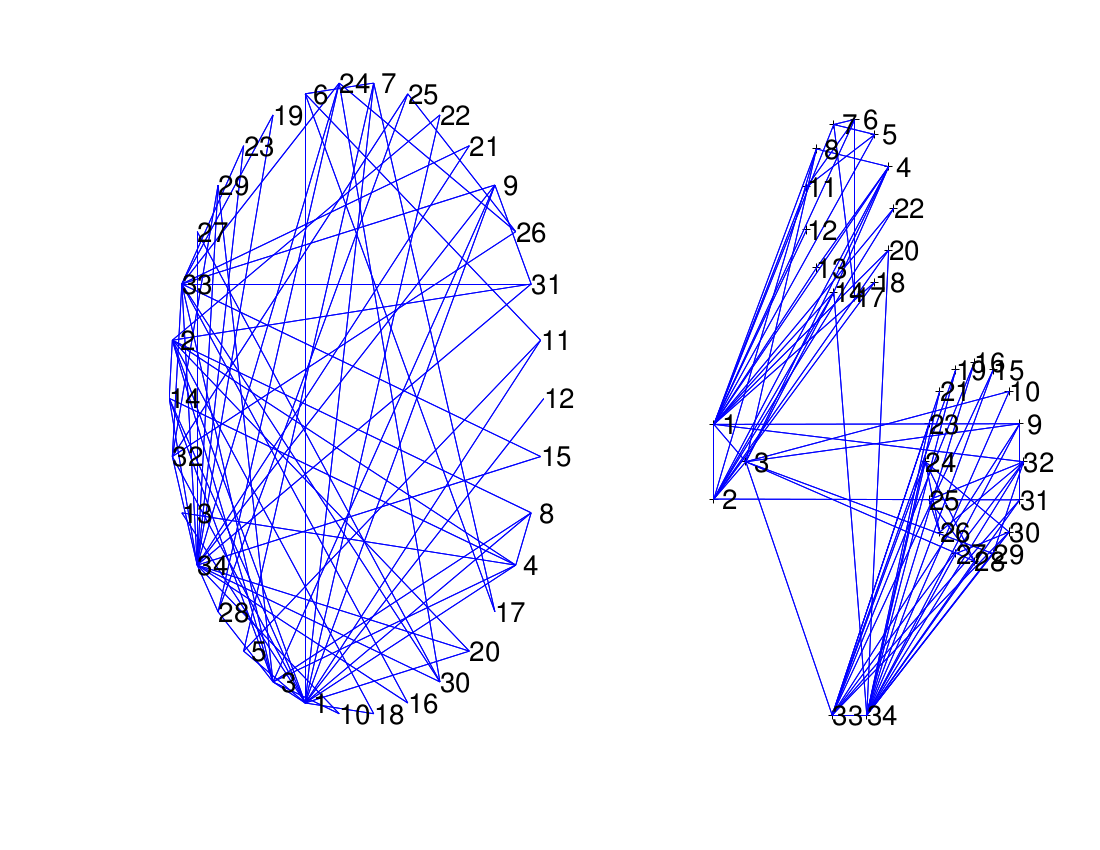
\epsfig{file = ../Figures/Karate-Graph.eps, clip=, width=7cm,
    height=20cm, angle=270}
  \\
  \epsfig{file = ../Figures/Karate-Dotplot.eps, clip=, width=7cm,
    height=20cm, angle=270}
\end{tabular}
$$

%%%%%%%%%%%%%%%%%%%%%%%%%%%%%%%%%%%%%%%%%%%%%%%%%%%%%%%%%%%%%%%%%%%%%
%%%%%%%%%%%%%%%%%%%%%%%%%%%%%%%%%%%%%%%%%%%%%%%%%%%%%%%%%%%%%%%%%%%%%
\newpage
\chapter{Random graphs}
%%%%%%%%%%%%%%%%%%%%%%%%%%%%%%%%%%%%%%%%%%%%%%%%%%%%%%%%%%%%%%%%%%%%%

\paragraph{Notation and definition.} Given a set of $n$ vertices ($i = 1..n$),
$X_{ij}$ indicates the presence/absence of a (non oriented) edge
between vertices $i$ and $j$:
$$
X_{ij} = X_{ji} = \Ibb\{i \leftrightarrow j\}, 
\qquad X_{ii} = 0.
$$
The random graph is defined by the join distribution of all the
$\{X_{ij}\}_{i, j}$.

%\vspace{1cm}
\paragraph{Typical characteristics.} 
\vspace{-0.5cm}
\begin{description}
\item[Degree of the vertices:] ${K_i = \sum_{j
      \neq i} X_{ij}}$ 
\item[Clustering coefficient:] ${c = \Pr\{X_{jk} = 1 \;|\;
    X_{ij} = X_{ik} = 1 \}}= \Pr\{\nabla \;|\; \Vsf\}$ 
\item[Diameter:] Longest path between two vertices.
\item[Number of occurrences of some motifs:] distribution of the
  number of triangles ($\nabla$), $\Vsf$, stars ({\Huge $\Starsf$}), etc.
\end{description}


%%%%%%%%%%%%%%%%%%%%%%%%%%%%%%%%%%%%%%%%%%%%%%%%%%%%%%%%%%%%%%%%%%%%%
%%%%%%%%%%%%%%%%%%%%%%%%%%%%%%%%%%%%%%%%%%%%%%%%%%%%%%%%%%%%%%%%%%%%%
\newpage
\chapter{Erd�s-R�nyi mixture for graph (ERMG)} \label{Sec:ErdosMixture}
%%%%%%%%%%%%%%%%%%%%%%%%%%%%%%%%%%%%%%%%%%%%%%%%%%%%%%%%%%%%%%%%%%%%%

\paragraph{Erd�s-R�nyi (ER) model.} $\{X_{ij}\}$ i.i.d.,  $\Pr\{ i
\leftrightarrow j\} = \pi$
$$
\Rightarrow \quad K_i \sim \Bcal(n-1, \pi) \approx \Pcal[(n-1)\pi],
\quad c = \pi.
$$
This model fits poorly many real-world networks, probably because
of some heterogeneity between the vertices.

% %%%%%%%%%%%%%%%%%%%%%%%%%%%%%%%%%%%%%%%%%%%%%%%%%%%%%%%%%%%%%%%%%%%%%
% \subsection{An explicit random graph model} 

\paragraph{Mixture population of edges.} We suppose that the
edges belong to $Q$ groups:
$$
\alpha_q = \Pr\{i \in q\}, 
\qquad
Z_{iq} = \Ibb\{i \in q\}.
$$
\paragraph{Conditional distribution of the edges.}
The edges $\{X_{ij}\}$ are conditionally independent given the group of
the vertices:
$$
X_{ij} \; |\; \{i \in q, j \in \ell \} \sim \Bcal(\pi_{q\ell}).
$$
$\pi_{q\ell} = \pi_{\ell q}$ is the connection probability between
groups $q$ and $\ell$. \\
A high value of $\pi_{q\ell}$ reveals a preferential connectivity
between groups $q$ and $\ell$. 

% \paragraph{Erd�s-R�nyi model.} The popular Erd�s-R�nyi fits
% poorly many real-world networks. It actually corresponds to $Q = 1$
% group. 

%%%%%%%%%%%%%%%%%%%%%%%%%%%%%%%%%%%%%%%%%%%%%%%%%%%%%%%%%%%%%%%%%%%%%
\newpage
%\subsection{Examples}
%%%%%%%%%%%%%%%%%%%%%%%%%%%%%%%%%%%%%%%%%%%%%%%%%%%%%%%%%%%%%%%%%%%%%
%$$
\hspace{-1cm} 
\begin{tabular}{lcccc}
  %\vspace{-3cm}
  \subsection{Examples} & Network & $Q$ & $\pi$ & Cluster. coef. \\
  \hline
  \begin{tabular}{p{2cm}} Random \end{tabular}
  & \begin{tabular}{c} \epsfig{file = ../figures/FigNetworks-Erdos-Col.eps,
      width=3.8cm, height=3.8cm, clip=, angle=270} 
  \end{tabular}
  & 1
  &  $p$ & $p$ \\
  \hline
  \begin{tabular}{p{2cm}} Independent model (product connectivity) \end{tabular}
  & \begin{tabular}{c} \epsfig{file = ../figures/FigNetworks-Indep-Col.eps,
      width=3.8cm, clip=, angle=270}
  \end{tabular}
  & 2
  & $\left( \begin{array}{cc} a^2 &ab\\ ab&b^2\\ \end{array}
  \right)$
  & $\displaystyle{\frac{(a^2+b^2)^2}{(a+b)^2}}$ \\
  \hline
  \begin{tabular}{p{2cm}} Stars \end{tabular}
  & \begin{tabular}{c} 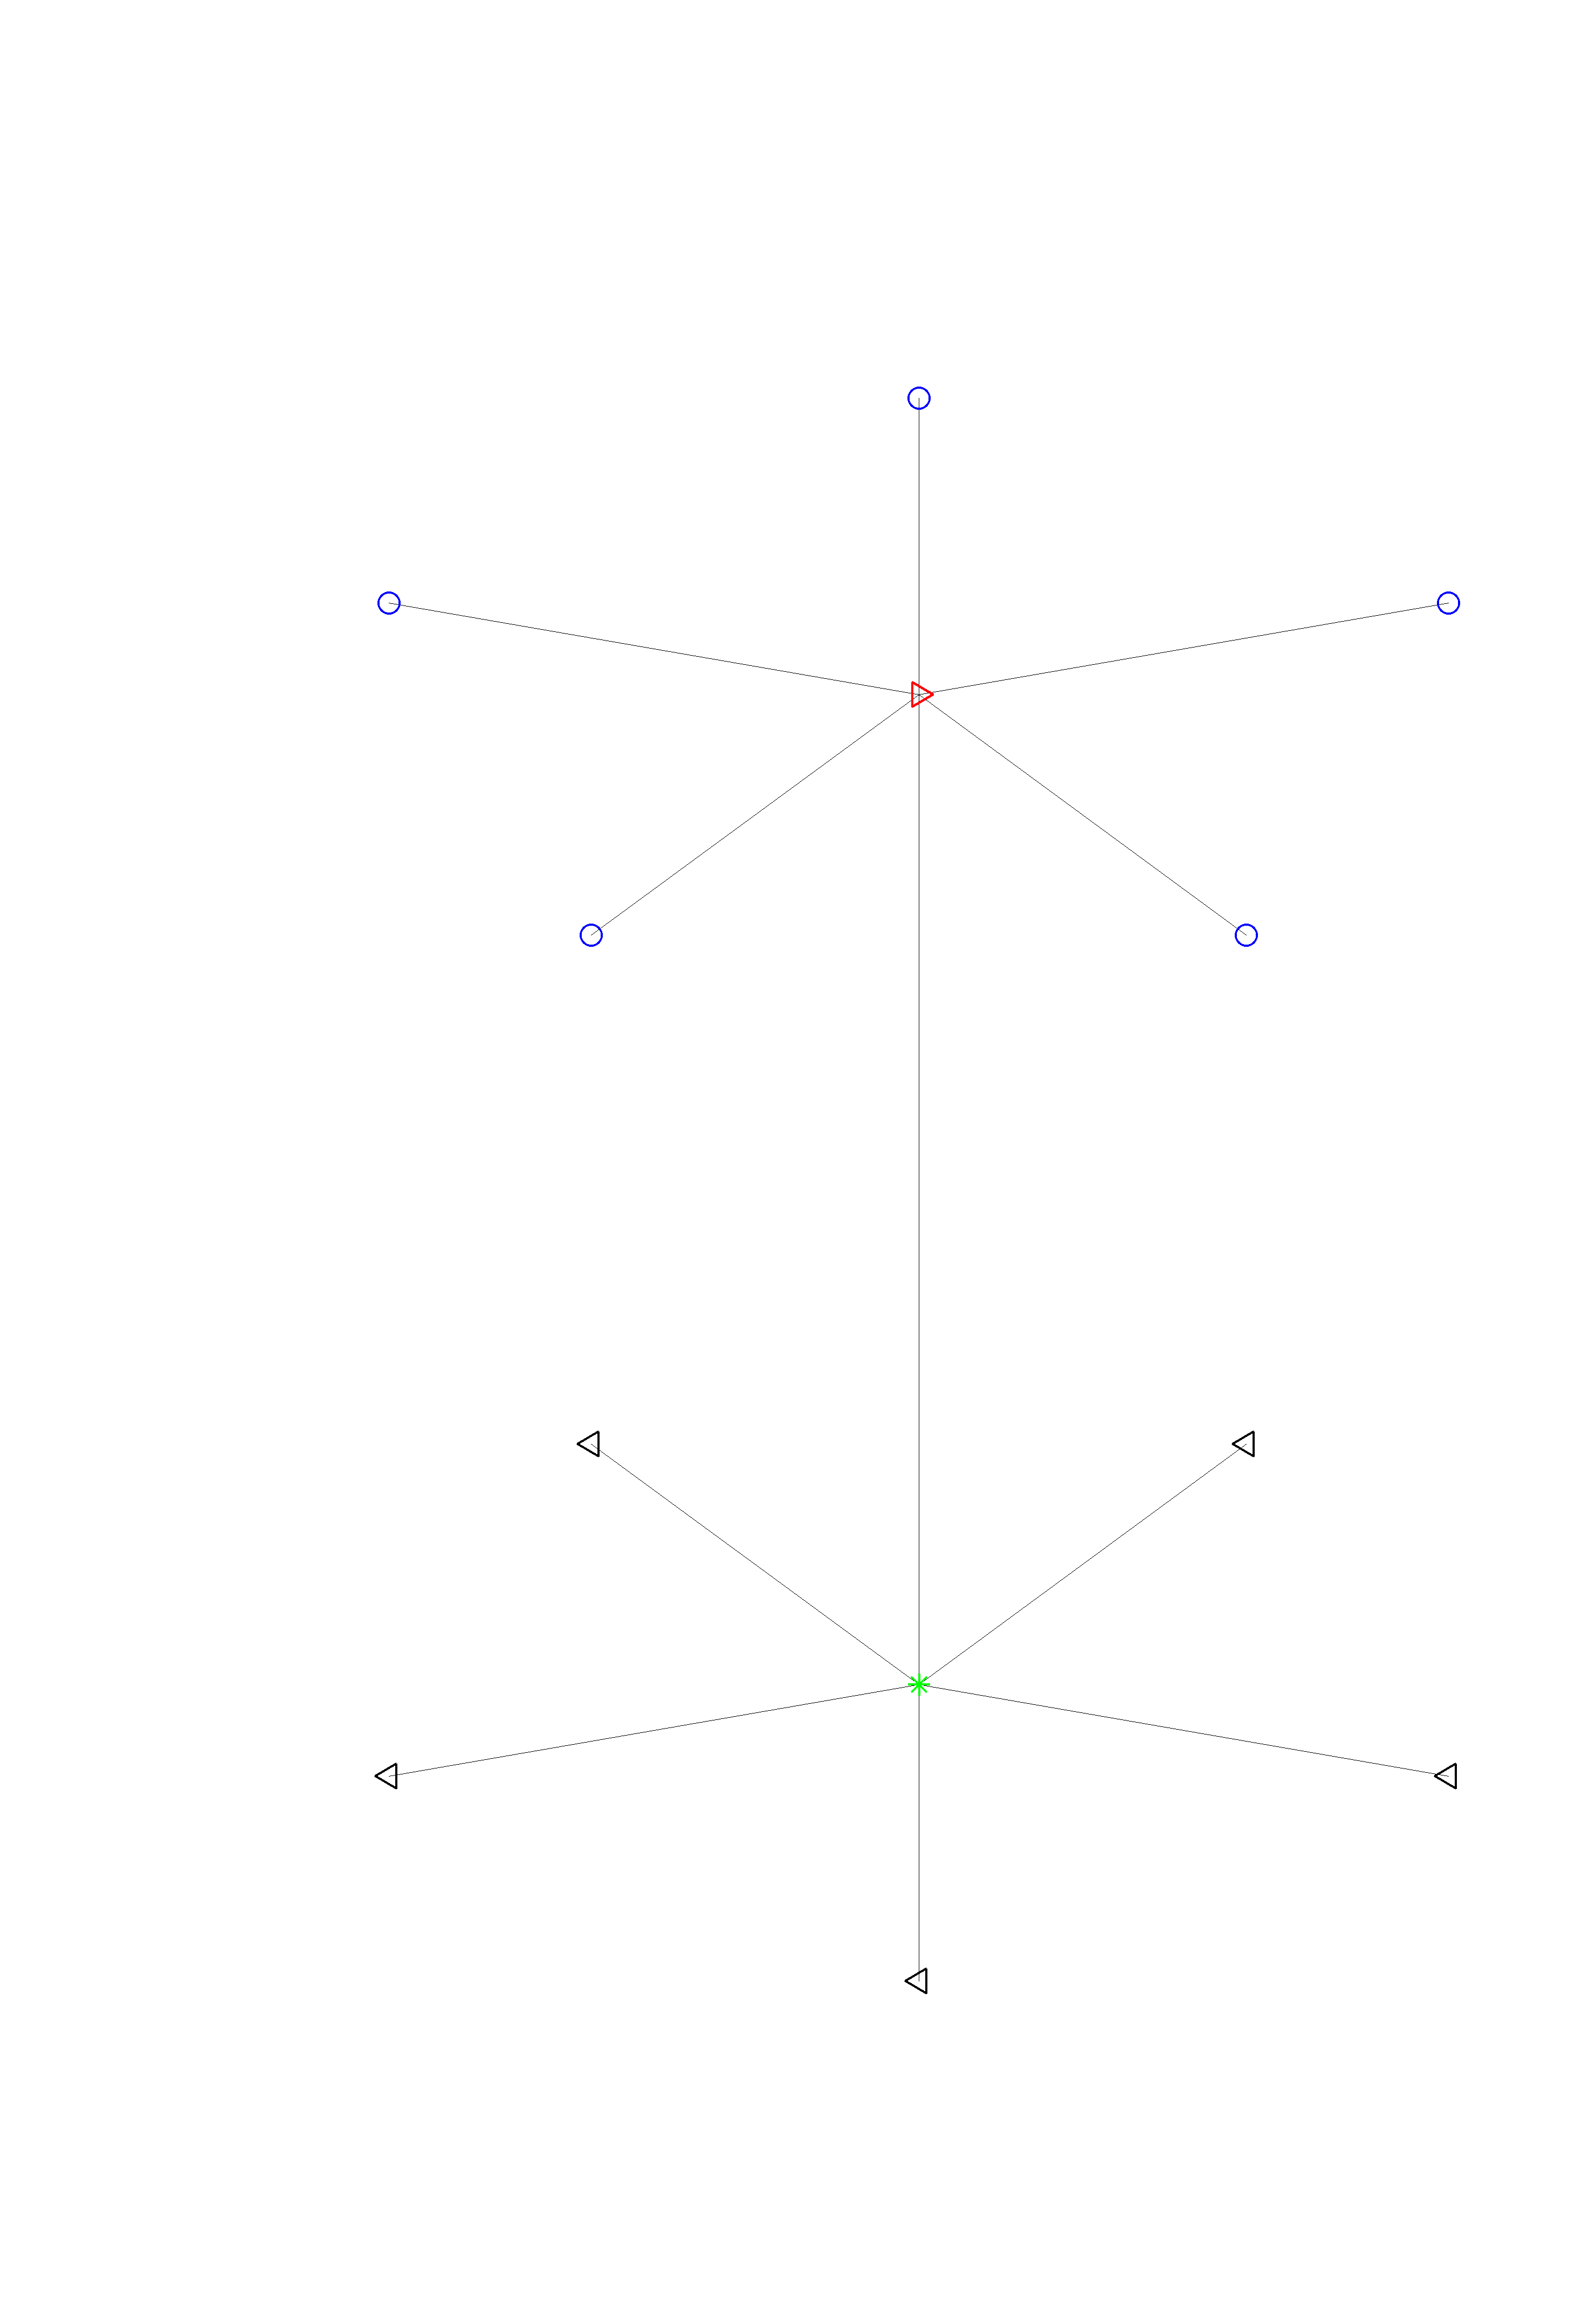
\epsfig{file = ../figures/FigNetworks-Star-Col.eps,
      width=3.8cm, clip=, angle=270}
  \end{tabular}
  & 4
  & $\left( \begin{array}{cccc} 0&1&0&0\\ 1&0&1&0\\0&1&0&1\\0&0&1&0\\
    \end{array} \right)$
  & 0 \\
  \hline \begin{tabular}{p{2cm}} Clusters (affiliation networks)
  \end{tabular} 
  & \begin{tabular}{c} \epsfig{file = ../figures/FigNetworks-Clusters-Col.eps,
      width=3.8cm, clip=, angle=270}
  \end{tabular}
  & 2
  & $\left(\begin{array}{cc} 1&\varepsilon\\ \varepsilon&1\\
    \end{array} \right)$ &
  $\displaystyle{\frac{1+3\varepsilon^2}{(1+\varepsilon)^2}}$ \\ 
\end{tabular} 
%$$
% \paragraph{Scale free network model }
%  (Barabasi \& Albert, 99) can also be expressed in terms of ERMG.

%%%%%%%%%%%%%%%%%%%%%%%%%%%%%%%%%%%%%%%%%%%%%%%%%%%%%%%%%%%%%%%%%%%%%
\newpage
\paragraph{Scale free distribution for the degree.}
Barabasi, Nat. Genet, 04
$$
p(k) = \Pr\{K = k\} \propto c k^{-(\rho+1)}
$$
$$
\epsfig{file = ../Figures/Barabasi4.ps, clip=, bbllx=0, bblly=304,
  bburx=595, bbury=688, width=21cm, height=14cm}
$$

%%%%%%%%%%%%%%%%%%%%%%%%%%%%%%%%%%%%%%%%%%%%%%%%%%%%%%%%%%%%%%%%%%%%%
\newpage
\paragraph{Scale free network model.}
(Barabasi \& Albert, 99)

The network is build iteratively: the $i$-th vertex joining the
network connects one of the $(i-1)$ preceeding ones with probability
proportional to their current degree (\paragraph{'busy gets busier'}):
$$
\forall j < i, \qquad \Pr\vspace{0cm}^i\{ i \leftrightarrow j\} \propto K_j^i.
$$
The limit marginal distribution of the degree is then scale free
(Zipf): $p(k) \propto k^{-3}$.

\bigskip\bigskip
\paragraph{Analogous modeling with the independent ERMG.} At time $q$,
$n_q = n \alpha_q$ vertices join the net work. They preferentially
connect the oldest vertices:
$$
\pi_{q\ell} = \eta_q \eta_{\ell}, 
\qquad \eta_1 \geq \eta_2 \geq \dots \geq \eta_q \geq \dots 
$$
The decreasing speed of the $\{\eta_q\}$ gives the tail of the degree
distribution. 

%%%%%%%%%%%%%%%%%%%%%%%%%%%%%%%%%%%%%%%%%%%%%%%%%%%%%%%%%%%%%%%%%%%%%
\newpage
\subsection{Some properties of the ERMG model}
%%%%%%%%%%%%%%%%%%%%%%%%%%%%%%%%%%%%%%%%%%%%%%%%%%%%%%%%%%%%%%%%%%%%%

\paragraph{Conditional distribution of the degree:} Denoting $
\pibar_q = \sum_{\ell} \alpha_{\ell} \pi_{q\ell}$, $\lambda_q = (n-1)
\pibar_q$
$$
K_i \;|\; \{i \in q \} \sim \Bcal(n-1, \pibar_q) \approx
\Pcal(\lambda_q).
$$
\bigskip\bigskip
\paragraph{Marginal distribution of the degree:} we get a Poisson mixture
$$
K_i \sim \sum_q \Bcal(n-1, \pibar_q) \approx \sum_q \alpha_q \Pcal(\lambda_q).
$$
%%%%%%%%%%%%%%%%%%%%%%%%%%%%%%%%%%%%%%%%%%%%%%%%%%%%%%%%%%%%%%%%%%%%%
%\newpage
\paragraph{Between-group connectivity.}
Let $A_{q\ell}$ denote the number of edges between groups $q$ and
$\ell$. Its expectation in the ERMG model is
$$
\Esp (A_{q\ell})  = \frac{n(n-1)}2 \alpha_q \alpha_{\ell} \pi_{q\ell}.
$$
\paragraph{Clustering coefficient:}  
$$
c = \Pr\{\nabla \;|\; \Vsf\} = \Pr\{\nabla\} / \Pr\{\Vsf\} 
= \frac{\sum_{q, \ell, m} \alpha_q \alpha_{\ell} \alpha_m \pi_{q\ell}
\pi_{qm} \pi_{\ell m}}{\sum_{q, \ell, m} \alpha_q
  \alpha_{\ell} \alpha_m \pi_{q\ell} \pi_{qm}}.
$$

%%%%%%%%%%%%%%%%%%%%%%%%%%%%%%%%%%%%%%%%%%%%%%%%%%%%%%%%%%%%%%%%%%%%%
\newpage
\chapter{Estimation of the parameters}
%%%%%%%%%%%%%%%%%%%%%%%%%%%%%%%%%%%%%%%%%%%%%%%%%%%%%%%%%%%%%%%%%%%%%

Denote $\Xcal$ the set of random edges and $\Zcal$ the set of labels.

The aim is to \paragraph{maximize the log-likelihood $\Lcal(\Xcal)$}
which is not calculable (need to sum over all possible $\Zcal$).  We
actually maximize
$$
\Jcal(R_{\Xcal}) = \Lcal(\Xcal) - \paragraph{KL\left[R_{\Xcal}(\Zcal),
  \Pr(\Zcal\:|\Xcal)\right]} = \Hcal(R_{\Xcal}) - \sum_{\Zcal}
R_{\Xcal}(\Zcal) \Lcal(\Xcal, \Zcal)
$$
where $\Hcal(R_{\Xcal})$ is the entropy of $R_{\Xcal}$:
$\Hcal(R_{\Xcal}) = -\sum_{\Zcal} R_{\Xcal}(\Zcal) \ln R_{\Xcal}(\Zcal)$.
  
The distribution $R_{\Xcal}(\Zcal)$ is chosen to be the
\paragraph{best approximation of $\Pr(\Zcal\:|\Xcal)$} in terms of
Kullback-Leibler ($KL$) distance:
$$
R_{\Xcal}(\Zcal) = \Pr(\Zcal\:|\Xcal) \quad \Rightarrow \quad
\Jcal(R_{\Xcal}) = \Lcal(\Xcal).
$$
\paragraph{Algorithm.} We alternately optimize $\Jcal(R_{\Xcal})$ with
respect \paragraph{($a$)} to $R_{\Xcal}$ and \paragraph{($b$)} to the
parameter estimates ($\widehat{\alpha}, \widehat{\pi}$), so the
proposed algorithm converges.

%%%%%%%%%%%%%%%%%%%%%%%%%%%%%%%%%%%%%%%%%%%%%%%%%%%%%%%%%%%%%%%%%%%%%
\newpage
\paragraph{($a$) Variational approach.}
We restrict the choice of $R_{\Xcal}$ to a 'comfortable' class: 
$$
R_{\Xcal}(\Zcal) = \prod_i h(\Zcal_i, \taubf_i)
\qquad  \Rightarrow \qquad 
\widehat{\tau}_{iq} \propto \alpha_q
  \prod_{\ell} b(\widehat{C}_{i\ell}; \widehat{N}^i_{\ell}, \pi_{q\ell})
\vspace{-0.5cm} 
$$
where
\begin{itemize}
\item \vspace{-0.5cm} $h$ is the multinomial distribution and
  $\taubf_i$'s are variational parameters to be optimized;
\item \vspace{-0.5cm} $b(c; n, \pi)$ denotes the binomial
  distribution, $\widehat{C}_{i\ell} = \sum_j
  \widehat{\tau}_{j\ell}X_{ij}$, $\widehat{N}^i_{\ell} = \sum_{j \neq i}
  \widehat{\tau}_{j\ell}$;  
\end{itemize}
The $\widehat{\tau}_{iq}$'s must satisfy the fix point relation: $
\widehat{\tau}_{iq} = \Pr\{Z_{iq} = 1 \;|\; \Xcal,
\widehat{\Zcal}^i\}$.

\noindent The $\widehat{\tau}_{iq}$'s turn out to be approximate conditional
expectations: $\widehat{\tau}_{iq} = \Esp_{R_{\Xcal}} Z_{iq}$ \\
$\Rightarrow \quad$ this corresponds to a \paragraph{'mean field'}
approximation.

\paragraph{($b$) Parameter estimates.}
Maximizing $\Jcal(R_{\Xcal})$ subject to $\sum_q \alpha_q = 1$ gives
$$
\widehat{\alpha}_q = \sum_i \widehat{\tau}_{iq} / n, \qquad
\widehat{\pi}_{q\ell} = \sum_i \sum_j \widehat{\tau}_{iq}\widehat{\tau}_{j\ell}
X_{ij} \left/ \sum_i \sum_j \widehat{\tau}_{iq}\widehat{\tau}_{j\ell} \right..
$$

%%%%%%%%%%%%%%%%%%%%%%%%%%%%%%%%%%%%%%%%%%%%%%%%%%%%%%%%%%%%%%%%%%%%%
\newpage
\subsection{Why not use the standard E-M algorithm?}

E-M is very popular to fit mixture models. It requires to calculate
the conditional distribution \paragraph{$\Pr\{\Zcal \;|\; \Xcal\}$}
which is intractable.
$$
\begin{tabular}{p{12cm}p{12cm}}
  \paragraph{Dependency graph} (oriented) & \paragraph{Moral graph}
  (parents are married) \\  
  \\
  Edge $X_{ij}$ only depends on its two parents $Z_1$ and $Z_2$
  &
  Conditional on the edges, labels $Z_i$'s all depend on each others \\
                                %\\
  \hspace{-1cm}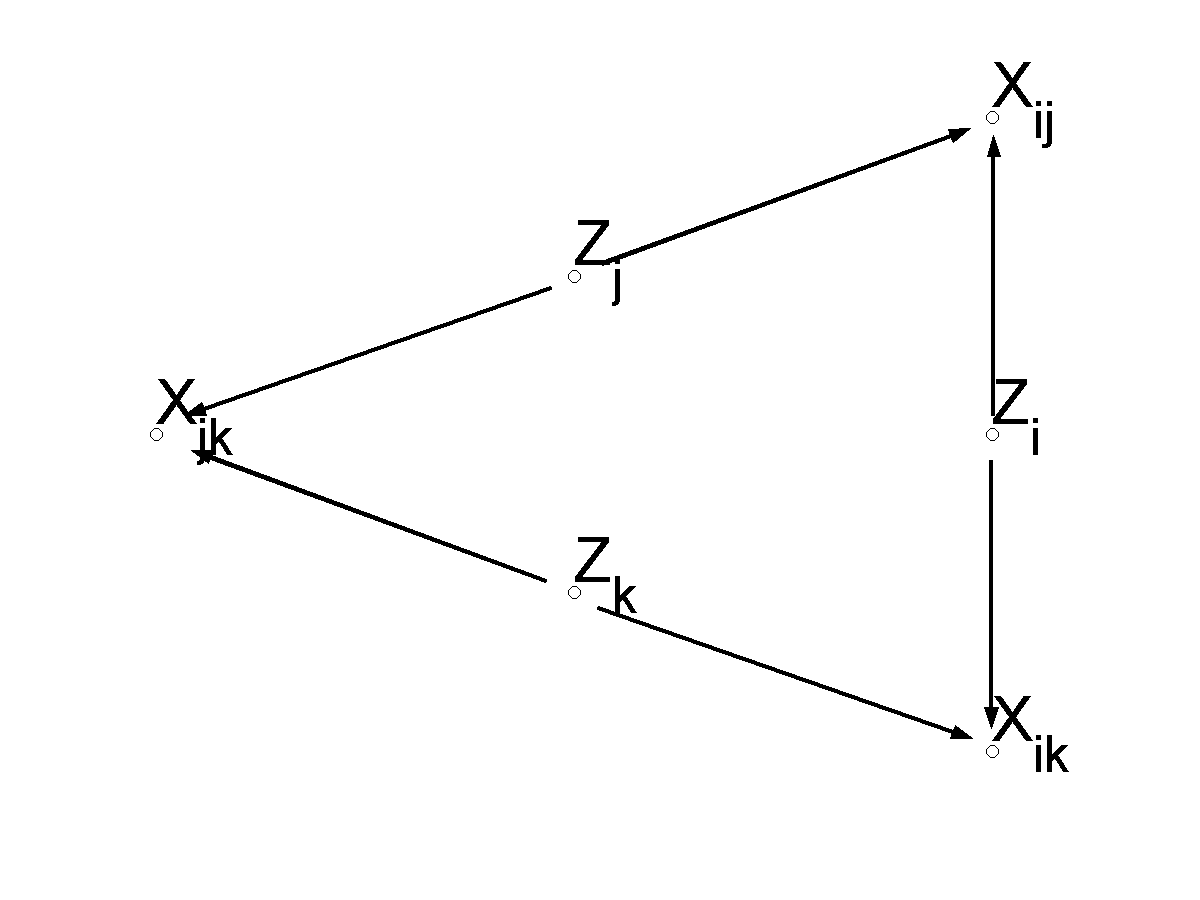
\epsfig{file = ../figures/FigNetworks-DepGraph.eps, clip=,
    angle=270, width=12cm}
  &
  \hspace{-1cm}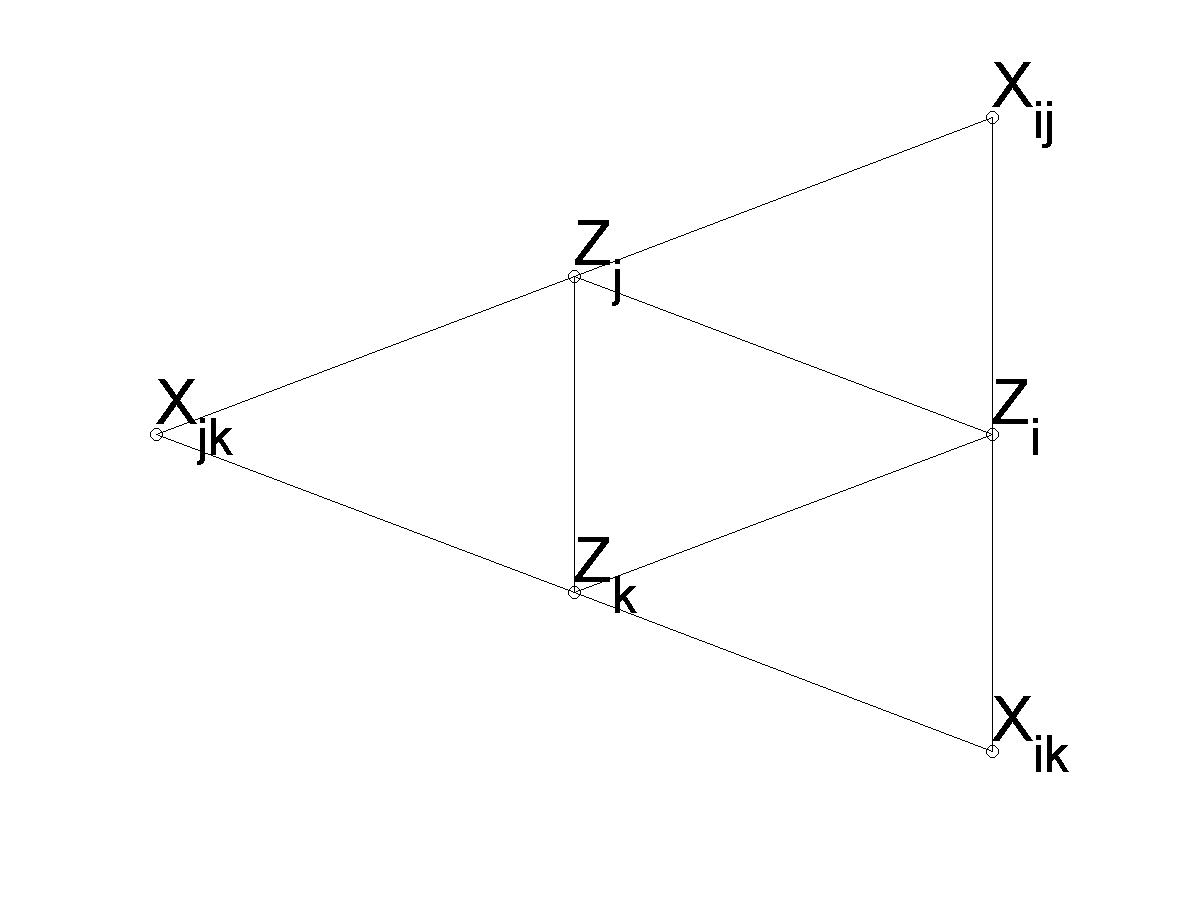
\epsfig{file = ../figures/FigNetworks-DepGraph-Moral.eps, clip=,
    angle=270, width=12cm} \\
  \multicolumn{2}{c}{\vspace{-0.5cm}$\Rightarrow$ All edges are actually 'neighbours'.}
\end{tabular}
$$

%%%%%%%%%%%%%%%%%%%%%%%%%%%%%%%%%%%%%%%%%%%%%%%%%%%%%%%%%%%%%%%%%%%%%
\newpage
\subsection{Choice of the number of groups}
%%%%%%%%%%%%%%%%%%%%%%%%%%%%%%%%%%%%%%%%%%%%%%%%%%%%%%%%%%%%%%%%%%%%%

We propose a heuristic penalized likelihood criterion inspired from
BIC.

The completed log-likelihood $\Lcal(\Xcal, \widehat{\Zcal})$ is the sum of
$$
\begin{tabular}{p{11cm}p{10cm}}
  $\displaystyle{\sum_i \sum_q \widehat{\tau}_{iq} \log \alpha_q}$ & 
  which deals with $(Q-1)$ independent proportions $\alpha_q$s and
  involves $n$ terms, 
  \\ 
  \\
  $\displaystyle{\sum_i \sum_q \sum_{j > i} \sum_{\ell}
  \widehat{\tau}_{iq}\widehat{\tau}_{j\ell} \log b(X_{ij};
  \pi_{q\ell})}$  
  & which deals with $Q(Q+1)/2$ probabilities $\pi_{q\ell}$s and
  involves $n(n-1)/2$ terms.
\end{tabular}
$$
We propose the following heuristic criterion:
$$
- 2\Lcal(\Xcal, \widehat{\Zcal}) + (Q-1) \log n + \frac{Q(Q+1)}2
\log\left[\frac{n(n-1)}2\right].
$$

%%%%%%%%%%%%%%%%%%%%%%%%%%%%%%%%%%%%%%%%%%%%%%%%%%%%%%%%%%%%%%%%%%%%%
\newpage
\chapter{Application to {\sl E. coli} reaction network}
%%%%%%%%%%%%%%%%%%%%%%%%%%%%%%%%%%%%%%%%%%%%%%%%%%%%%%%%%%%%%%%%%%%%%
\begin{itemize}
\item \vspace{-0.5cm} $n = 605$ vertices (reactions) and $1\;782$
  edges. 
\item \vspace{-0.5cm} 2 reactions $i$ and $j$ are connected if the
  product of $i$ is the substrate of $j$ (or conversely).
\item \vspace{-0.5cm} provided by V. Lacroix and M.-F. Sagot (INRIA
H�lix).
\end{itemize}

\subsection{Distribution of the degree}

\paragraph{Parameter estimates.} The BIC criterion select $Q = 3$ groups:
$$
\begin{tabular}{cccc}
  group & 1 & 2 & 3 \\
  \hline
  $\widehat{\alpha}$ (\%) & 8.9 & 19.7 & 71.3 \\
  $\widehat{\lambda}$ & 21.5 & 9.1 & 3.0 \\
\end{tabular}
$$

%%%%%%%%%%%%%%%%%%%%%%%%%%%%%%%%%%%%%%%%%%%%%%%%%%%%%%%%%%%%%%%%%%%%%
\newpage
\paragraph{Distribution plots.} 
$$
\begin{tabular}{cccc}
  Distribution & log-log plot & histogram & P-P plot \\ 
%  \\
  \hline
  \begin{tabular}{c} Zipf \end{tabular}
  & \begin{tabular}{c} \epsfig{file = ../figures/log-log.eps,
      height=5cm, width = 5cm} \end{tabular}
  & \begin{tabular}{c} 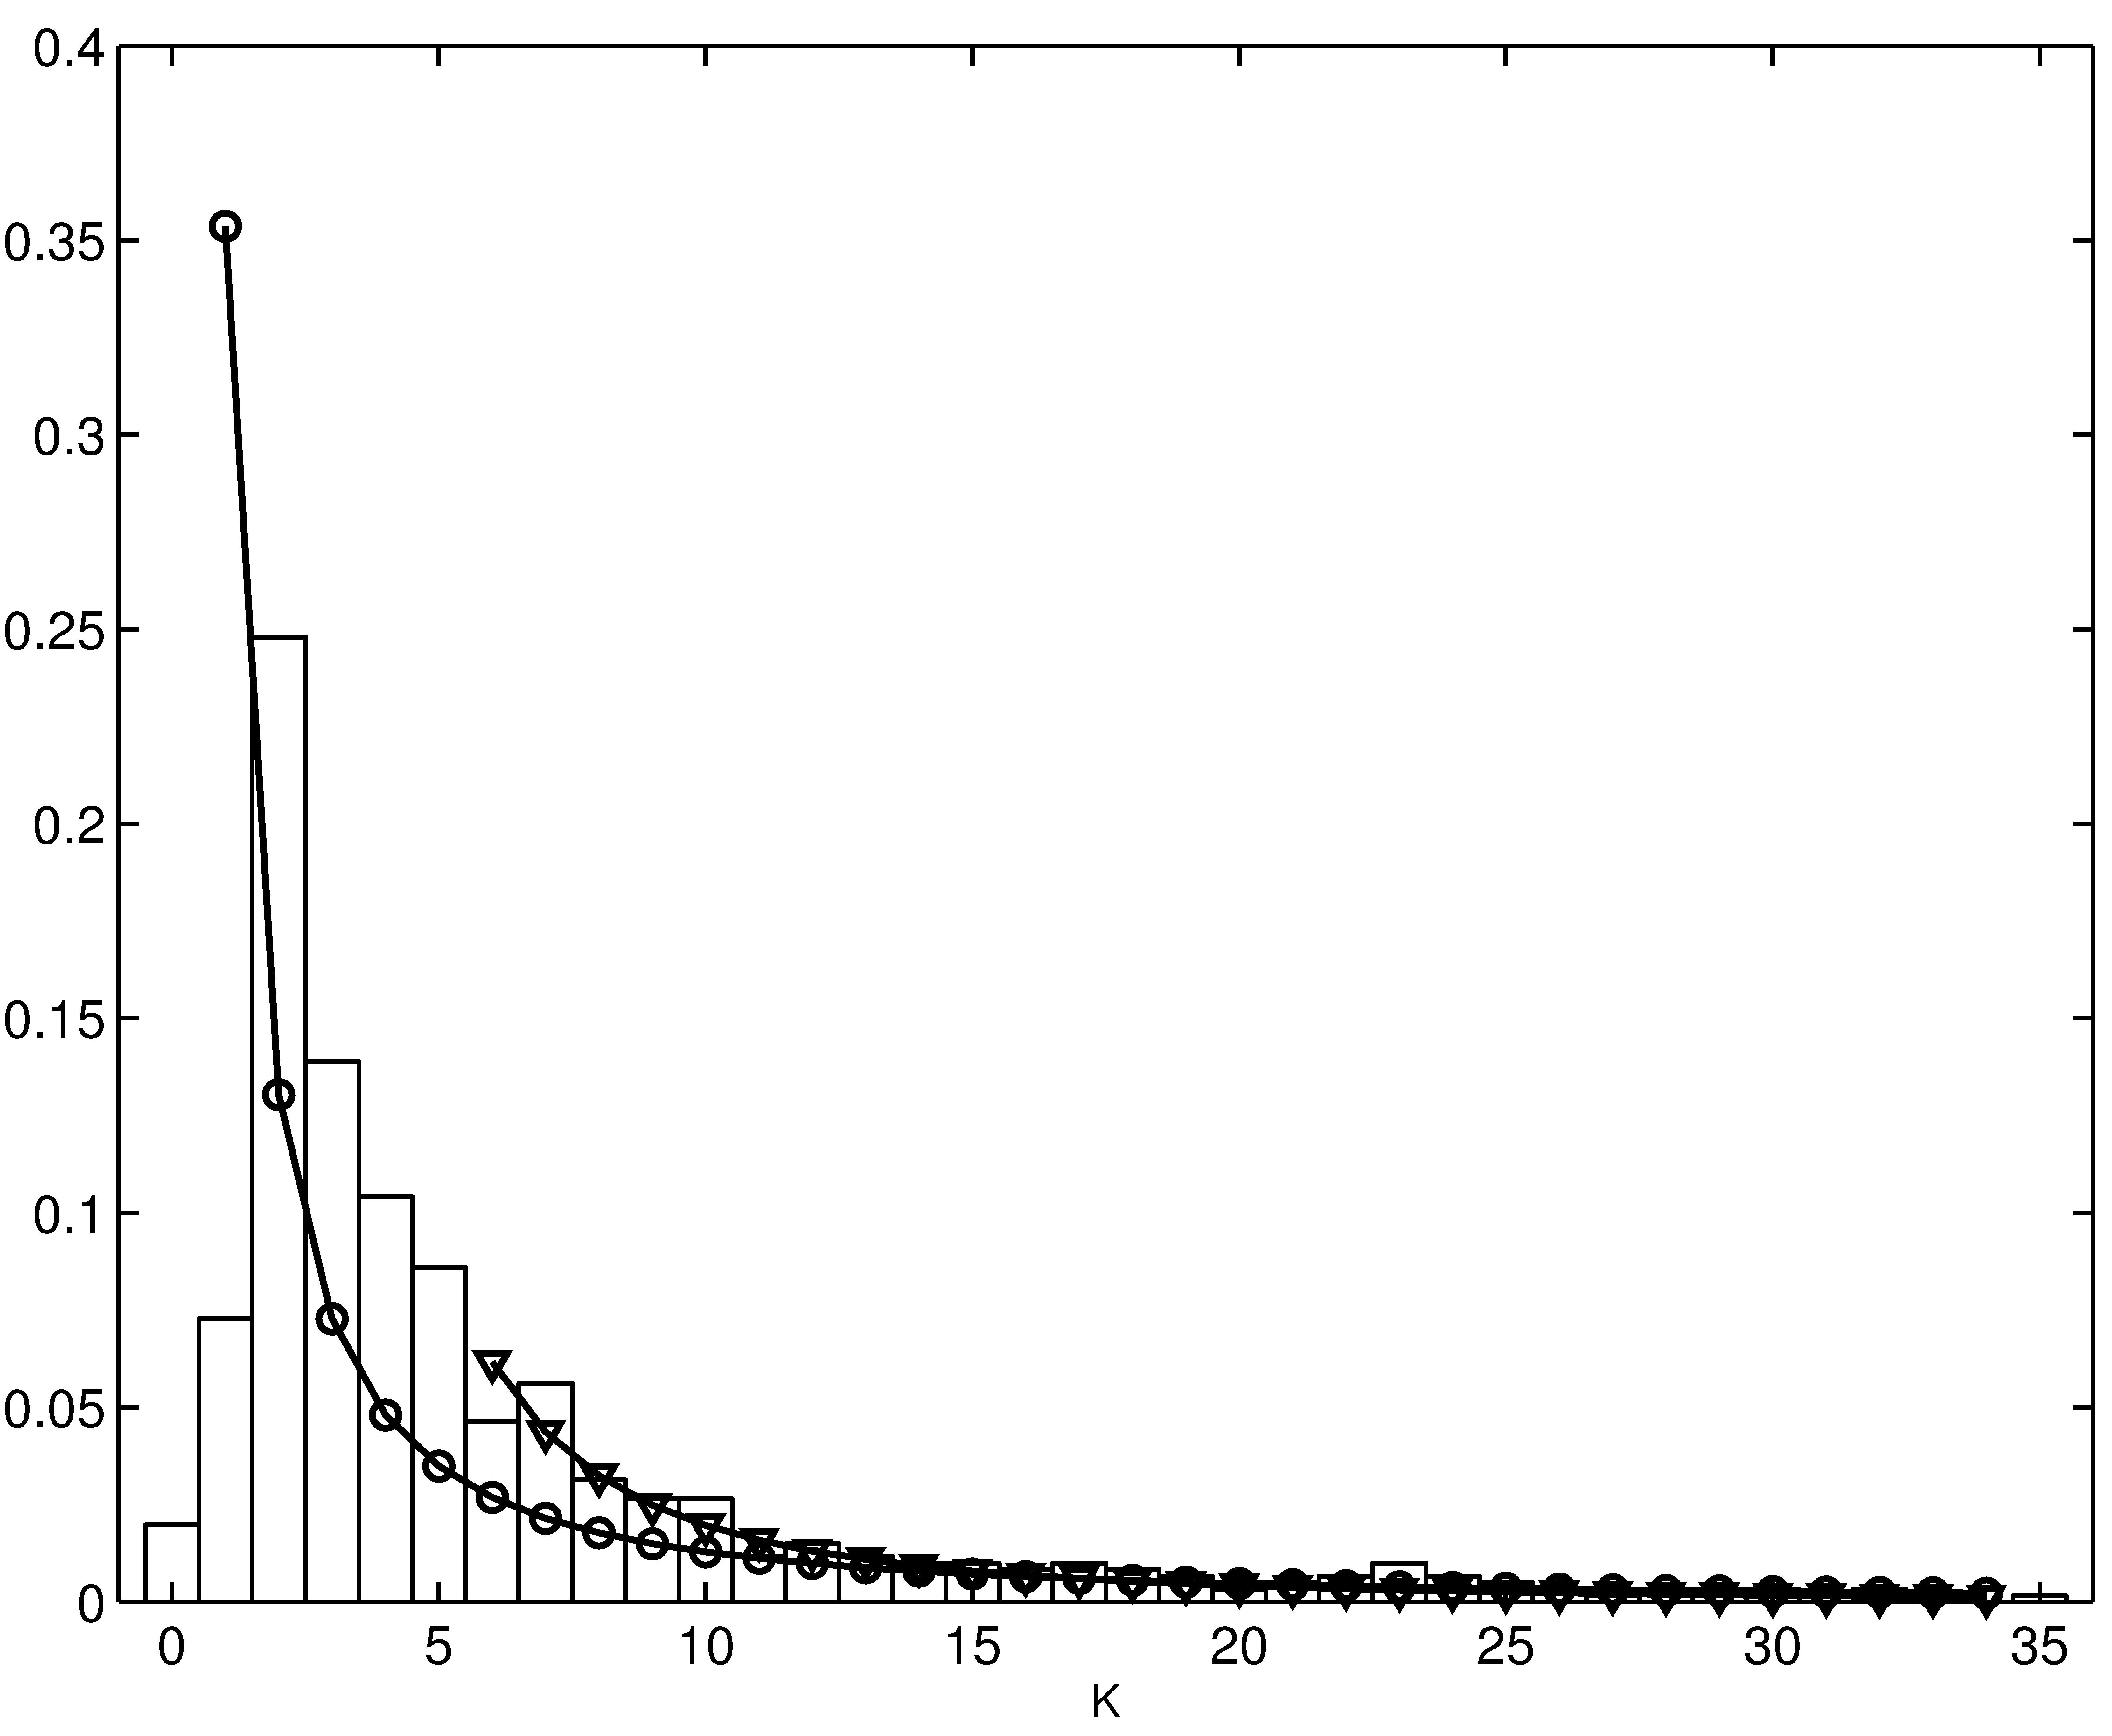
\epsfig{file = ../figures/histo_degre_power.eps,
      height=5cm, width = 5cm} \end{tabular}
  & \begin{tabular}{c} \epsfig{file = ../figures/pp-plot-power.eps,
      height=5cm, width = 5cm} \end{tabular} \\ 
%  & & threshold = 1 & threshold = 6 \\
  \hline
%  \\
  \begin{tabular}{c} Poisson \\ mixture \end{tabular}
   & & \begin{tabular}{c} 
    %\epsfig{file = ../figures/degre_melange.eps, height=5cm, width=5cm} 
    \epsfig{file = ../figures/ECOli-Poisson-Q3.eps, height=5cm,
    width=5cm, angle=90, bbllx=335, bblly=415, bburx=555, bbury=700, clip=}  
  \end{tabular}
  & \begin{tabular}{c} 
    %\epsfig{file = ../figures/PPplot_melange.eps, height=5cm, width=5cm} 
    \epsfig{file = ../figures/ECOli-Poisson-Q3.eps, height=5cm,
    width=5cm, angle=90, bbllx=65, bblly=80, bburx=285, bbury=360, clip=} 
  \end{tabular} \\
\end{tabular}
$$

%%%%%%%%%%%%%%%%%%%%%%%%%%%%%%%%%%%%%%%%%%%%%%%%%%%%%%%%%%%%%%%%%%%%%
\newpage
\paragraph{Fit statistics.} The Zipf distribution is only defined
above a certain threshold. 
$$
\begin{tabular}{ccccccccc}
  & & \multicolumn{4}{c}{Power law} & \multicolumn{3}{c}{Poisson mixture} \\
  Threshold & $n$ & $\rho+1$ & $\chi^2$ stat. & df & $p$-value
  & $\chi^2$ stat. & df & $p$-value \\
  \hline
  0 & 593 & -    & -     & -  & -            & 67.25 & 29 & $7\;10^{-5}$\\
  1 & 549 & 1.79 & 96.22 & 32 & $2\;10^{-9}$ & 58.5  & 28 & $6\;10^{-4}$\\
  2 & 399 & 1.93 & 75.83 & 31 & $1\;10^{-6}$ & 32.3  & 27 & $0.22$\\
  3 & 315 & 2.08 & 59.70 & 30 & $0.001     $ & 30.6  & 26 & $0.24$\\
  4 & 252 & 2.19 & 53.07 & 29 & $0.004     $ & 27.0  & 25 & $0.36$\\
  5 & 200 & 2.24 & 52.37 & 28 & $0.003     $ & 27.0  & 24 & $0.30$\\
  6 & 172 & 2.37 & 45.44 & 27 & $0.014     $ & 25.0  & 23 & $0.35$\\
\end{tabular}
$$

\paragraph{Preliminary conclusions.}
\begin{itemize}
\item \vspace{-0.5cm} The Poisson mixture fits the data well, better
  than the Zipf model.
\item \vspace{-0.5cm} \paragraph{\sl But a model for the degrees is not a model for
  the graph}.
\end{itemize}

%%%%%%%%%%%%%%%%%%%%%%%%%%%%%%%%%%%%%%%%%%%%%%%%%%%%%%%%%%%%%%%%%%%%%
\newpage
\subsection{Mixture model for the graph: ERMG} 

\paragraph{Number of groups.} Pseudo-BIC selects $Q = 21$. 

% \paragraph{Parameter estimates.} \\
% ${\tiny
%   \begin{array}{cccccccccccccccccccccc}
%     \hline
%     \alpha (\%) & 0.7 & 1.0 & 1.2 & 1.3 & 1.3 & 1.5 & 1.5 & 1.6 &
%     1.8 & 1.8 & 2.0 & 2.1 & 2.3 & 2.6 & 2.7 & 2.8 & 3.0 & 3.0 & 3.3
%     & 5.8 & 56.8 \\ 
%     \hline
%     & 100 & & & & & & 64 & & 11 & 43 & & & 2 & & & 100 & & & & & \\ 
%     & & 100 & & & & & & & & & & & & & & & & & & & \\ 
%     & & & 100 & & & & & & & & & 4 & 7 & & 1 & & & 1 & & & \\ 
%     & & & & 71 & & & & & & & & & & & & & & & & & \\ 
%     & & & & & 100 & 28 & & & & 1 & & & & & & 18 & & & 16 & & \\ 
%     & & & & & 28 & 100 & & & & & & & & 6 & & & & & & & \\ 
%     & 64 & & & & & & 58 & & 10 & 4 & & 7 & 5 & & & 5 & & & & & \\ 
%     & & & & & & & & 63 & & & & 5 & & & & & & 3 & & & \\ 
%     & 11 & & & & & & 10 & & 65 & & & & & & & 1 & 2 & 2 & & & \\ 
%     & 43 & & & & 1 & & 4 & & & 67 & & & 1 & & & & & & & & \\ 
%     \pi & & & & & & & & & & & 62 & & & 7 & & & 4 & & & & \\ 
%     (\%) & & & 4 & & & & 7 & 5 & & & & 28 & 5 & & & 5 & & & & & \\ 
%     & 2 & & 7 & & & & 5 & & & 1 & & 5 & 100 & & & 1 & & & & & \\ 
%     & & & & & & 6 & & & & & 7 & & & 25 & & & & & & & \\ 
%     & & & 1 & & & & & & & & & & & & 40 & & & & & & \\ 
%     & 100 & & & & 18 & & 5 & & 1 & & & 5 & 1 & & & 100 & & & & & \\ 
%     & & & & & & & & & 2 & & 4 & & & & & & 100 & & & 6 & \\ 
%     & & & 1 & & & & & 3 & 2 & & & & & & & & & 21 & & & \\ 
%     & & & & & 16 & & & & & & & & & & & & & & 19 & & \\ 
%     & & & & & & & & & & & & & & & & & 6 & & & 11 & \\  
%     & & & & & & & & & & & & & & & & & & & & & 1 \\ 
%     \hline
%     \lambda_q & 33 & 7 & 9 & 6 & 17 & 13 & 12 & 7 & 10 & 10 & 10 & 8
%     & 17 & 6 & 7 & 25 & 21 & 5 & 6 & 5 & 3 \\
%     \hline
%   \end{array}
%   }$

\paragraph{Group proportions.} $\widehat{\alpha}_q$ (\%).
$$
\vspace{-.5cm}
\epsfig{file = ../figures/Ecoli-Complet-ERMG-Ward-Q21_param.eps, height=6cm,
  width=12cm, clip=, bbllx=75, bblly=570, bburx=530, bbury=770}  
$$
\vspace{-.5cm}
Many small groups actually correspond to cliques or pseudo-cliques.

% \paragraph{Clustering coefficient.}
% $$
% \begin{tabular}{cccc}
%   Empirical & ERMG ($Q = 6$) & ERMG ($Q = 21$) & ER ($Q = 1$)\\
%   \hline
%   0.626 & 0.436 & 0.544 & 0.0098
% \end{tabular}
% $$

%%%%%%%%%%%%%%%%%%%%%%%%%%%%%%%%%%%%%%%%%%%%%%%%%%%%%%%%%%%%%%%%%%%%%
\newpage
\hspace{-2cm}
\begin{tabular}{cc}
  \begin{tabular}{p{11cm}}
    \paragraph{Dot-plot representation of the graph.} \\ \\ \\
    \paragraph{Biological interpretation:} Groups 1 to 20 gather
    reactions involving all the  same compound either as a substrate or as a
    product. \\ \\
    A compound (chorismate, pyruvate, ATP, {\sl etc}) can be associated to each
    group. \\ \\ \\
  \end{tabular}
  &
  \begin{tabular}{c}
    \epsfig{file = ../figures/Ecoli-Complet-ERMG-Ward-Q21_class.eps,
      height=13cm, width=13cm, clip=,bbllx=70, bblly=440, bburx=540,
      bbury=770}   
  \end{tabular} 
  \vspace{-1cm}
  \\
  \begin{tabular}{p{11cm}}
    \paragraph{Posterior probabilities $\widehat{\tau}_{iq}$.}  \\ \\ \\
  \end{tabular}
  & 
  \begin{tabular}{c}
    \epsfig{file = ../figures/Ecoli-Complet-ERMG-Ward-Q21_class.eps,
    width=13cm, clip=, bbllx=70, bblly=265, bburx=540, bbury=420}  
  \end{tabular}
\end{tabular}
%$$

%%%%%%%%%%%%%%%%%%%%%%%%%%%%%%%%%%%%%%%%%%%%%%%%%%%%%%%%%%%%%%%%%%%%%
\newpage
\hspace{-2cm}
\begin{tabular}{cc}
  \begin{tabular}{p{9cm}}
    \paragraph{Zoom (bottom left).} \\ 
    \\
    Submatrix of $\pi$:
    $$
    \begin{tabular}{c|cccc}
      $q, \ell$ & 1 & 7 & 10 & 16 \\
      \hline 
      1 & \paragraph{\bf 1.0} \\ 
      7 & \paragraph{\sl .11} & .65 \\ 
      10 & \paragraph{\sl .43} & & .67  \\ 
      16 & \paragraph{\bf 1.0} & \paragraph{\sl .01} & & \paragraph{\bf 1.0} \\
    \end{tabular}
    $$
    Groups 1 and 16 both involve pyruvate, but only group 1 involves also
    CO2 (group 7) and acetylCoA (group 10).
    \\ \\ 
  \end{tabular}
  &
  \begin{tabular}{l}
    \hspace{1.3cm}
    \epsfig{file = ../figures/Ecoli-Complet-ERMG-Ward-Q21_class.eps,
      height=12cm, width=12cm, clip=,bbllx=90, bblly=485, bburx=277,
      bbury=605.5}   
  \end{tabular}  
  \vspace{-2cm}
  \\ \\ \\
  \begin{tabular}{p{9cm}}
    \paragraph{Vertices degree $K_i$.}  \\ \\ 
    Mean degree in the last group:\\ 
    $\overline{K}_{21} = 2.6$ \\ \\ \\
  \end{tabular}
  & 
  \begin{tabular}{l}
    \epsfig{file = ../figures/Ecoli-Complet-ERMG-Ward-Q21_class.eps,
    width=13.4cm, height=6cm, clip=, bbllx=70, bblly=105, bburx=277,
    bbury=245}   
  \end{tabular}
\end{tabular}

%%%%%%%%%%%%%%%%%%%%%%%%%%%%%%%%%%%%%%%%%%%%%%%%%%%%%%%%%%%%%%%%%%%%%
\newpage
%\hspace{-2cm}
% \begin{tabular}{ll}
%   \begin{tabular}{p{11cm}}
%     \paragraph{Between group connectivity.} \\
%     Observed vs predicted: quite good \\ \\ 
%     but the 'observed' $A_{q\ell}$ are not observed but estimated with the MAP
%     rule:
%     $$
%     {\widehat{A}_{q\ell} = \sum_{i<j} \widehat{Z}_{iq}
%       \widehat{Z}_{j\ell} X_{ij}}
%     $$
%     so the observed good fit is optimistic. \\ \\ \\
%   \end{tabular}
%   & 
%   \begin{tabular}{c}
%     \epsfig{file =
%       ../figures/Ecoli-Complet-ERMG-Ward-Q21_param.eps, height=10cm,
%       width=10cm, clip=, bbllx=70, bblly=300, bburx=530, bbury=530}   
%   \end{tabular}
% \end{tabular}
\subsection{Model Fit}

\paragraph{Distribution of the degree.} According to the ERMG, the
      degrees have a Poisson mixture distribution with 21 components.
$$
\vspace{-1cm}
\begin{tabular}{cc}
  Histogram + mixture distribution & P-P plot \\
  \multicolumn{2}{c}{
    \epsfig{file =
      ../figures/Ecoli-Complet-ERMG-Ward-Q21_degree.eps, height=8cm,
      width=20cm, clip=, bbllx=80, bblly=210, bburx=550, bbury=590}   
    }
\end{tabular}
$$

\paragraph{Clustering coefficient.}
$$
\begin{tabular}{cccc}
  Empirical & ERMG ($Q = 6$) & ERMG ($Q = 21$) & ER ($Q = 1$)\\
  \hline
  0.626 & 0.436 & 0.544 & 0.0098
\end{tabular}
$$

%%%%%%%%%%%%%%%%%%%%%%%%%%%%%%%%%%%%%%%%%%%%%%%%%%%%%%%%%%%%%%%%%%%%%%%%
\newpage
\chapter{Using ERMG for Motif Statistics} 
\vspace{0.5cm}
\centerline{\sl Joint work with E. Birmele, C. Matias (Evry), E. Roquain,
  S. Schbath (Jouy-en-Josas)}

The organisation of a network can be charaterized by the frequency of some
\paragraph{specific motifs}:
$$
\begin{tabular}{cccccc}
  \begin{tabular}{c} Chain: \end{tabular} & 
  \begin{tabular}{c} \hspace{-1.5cm} 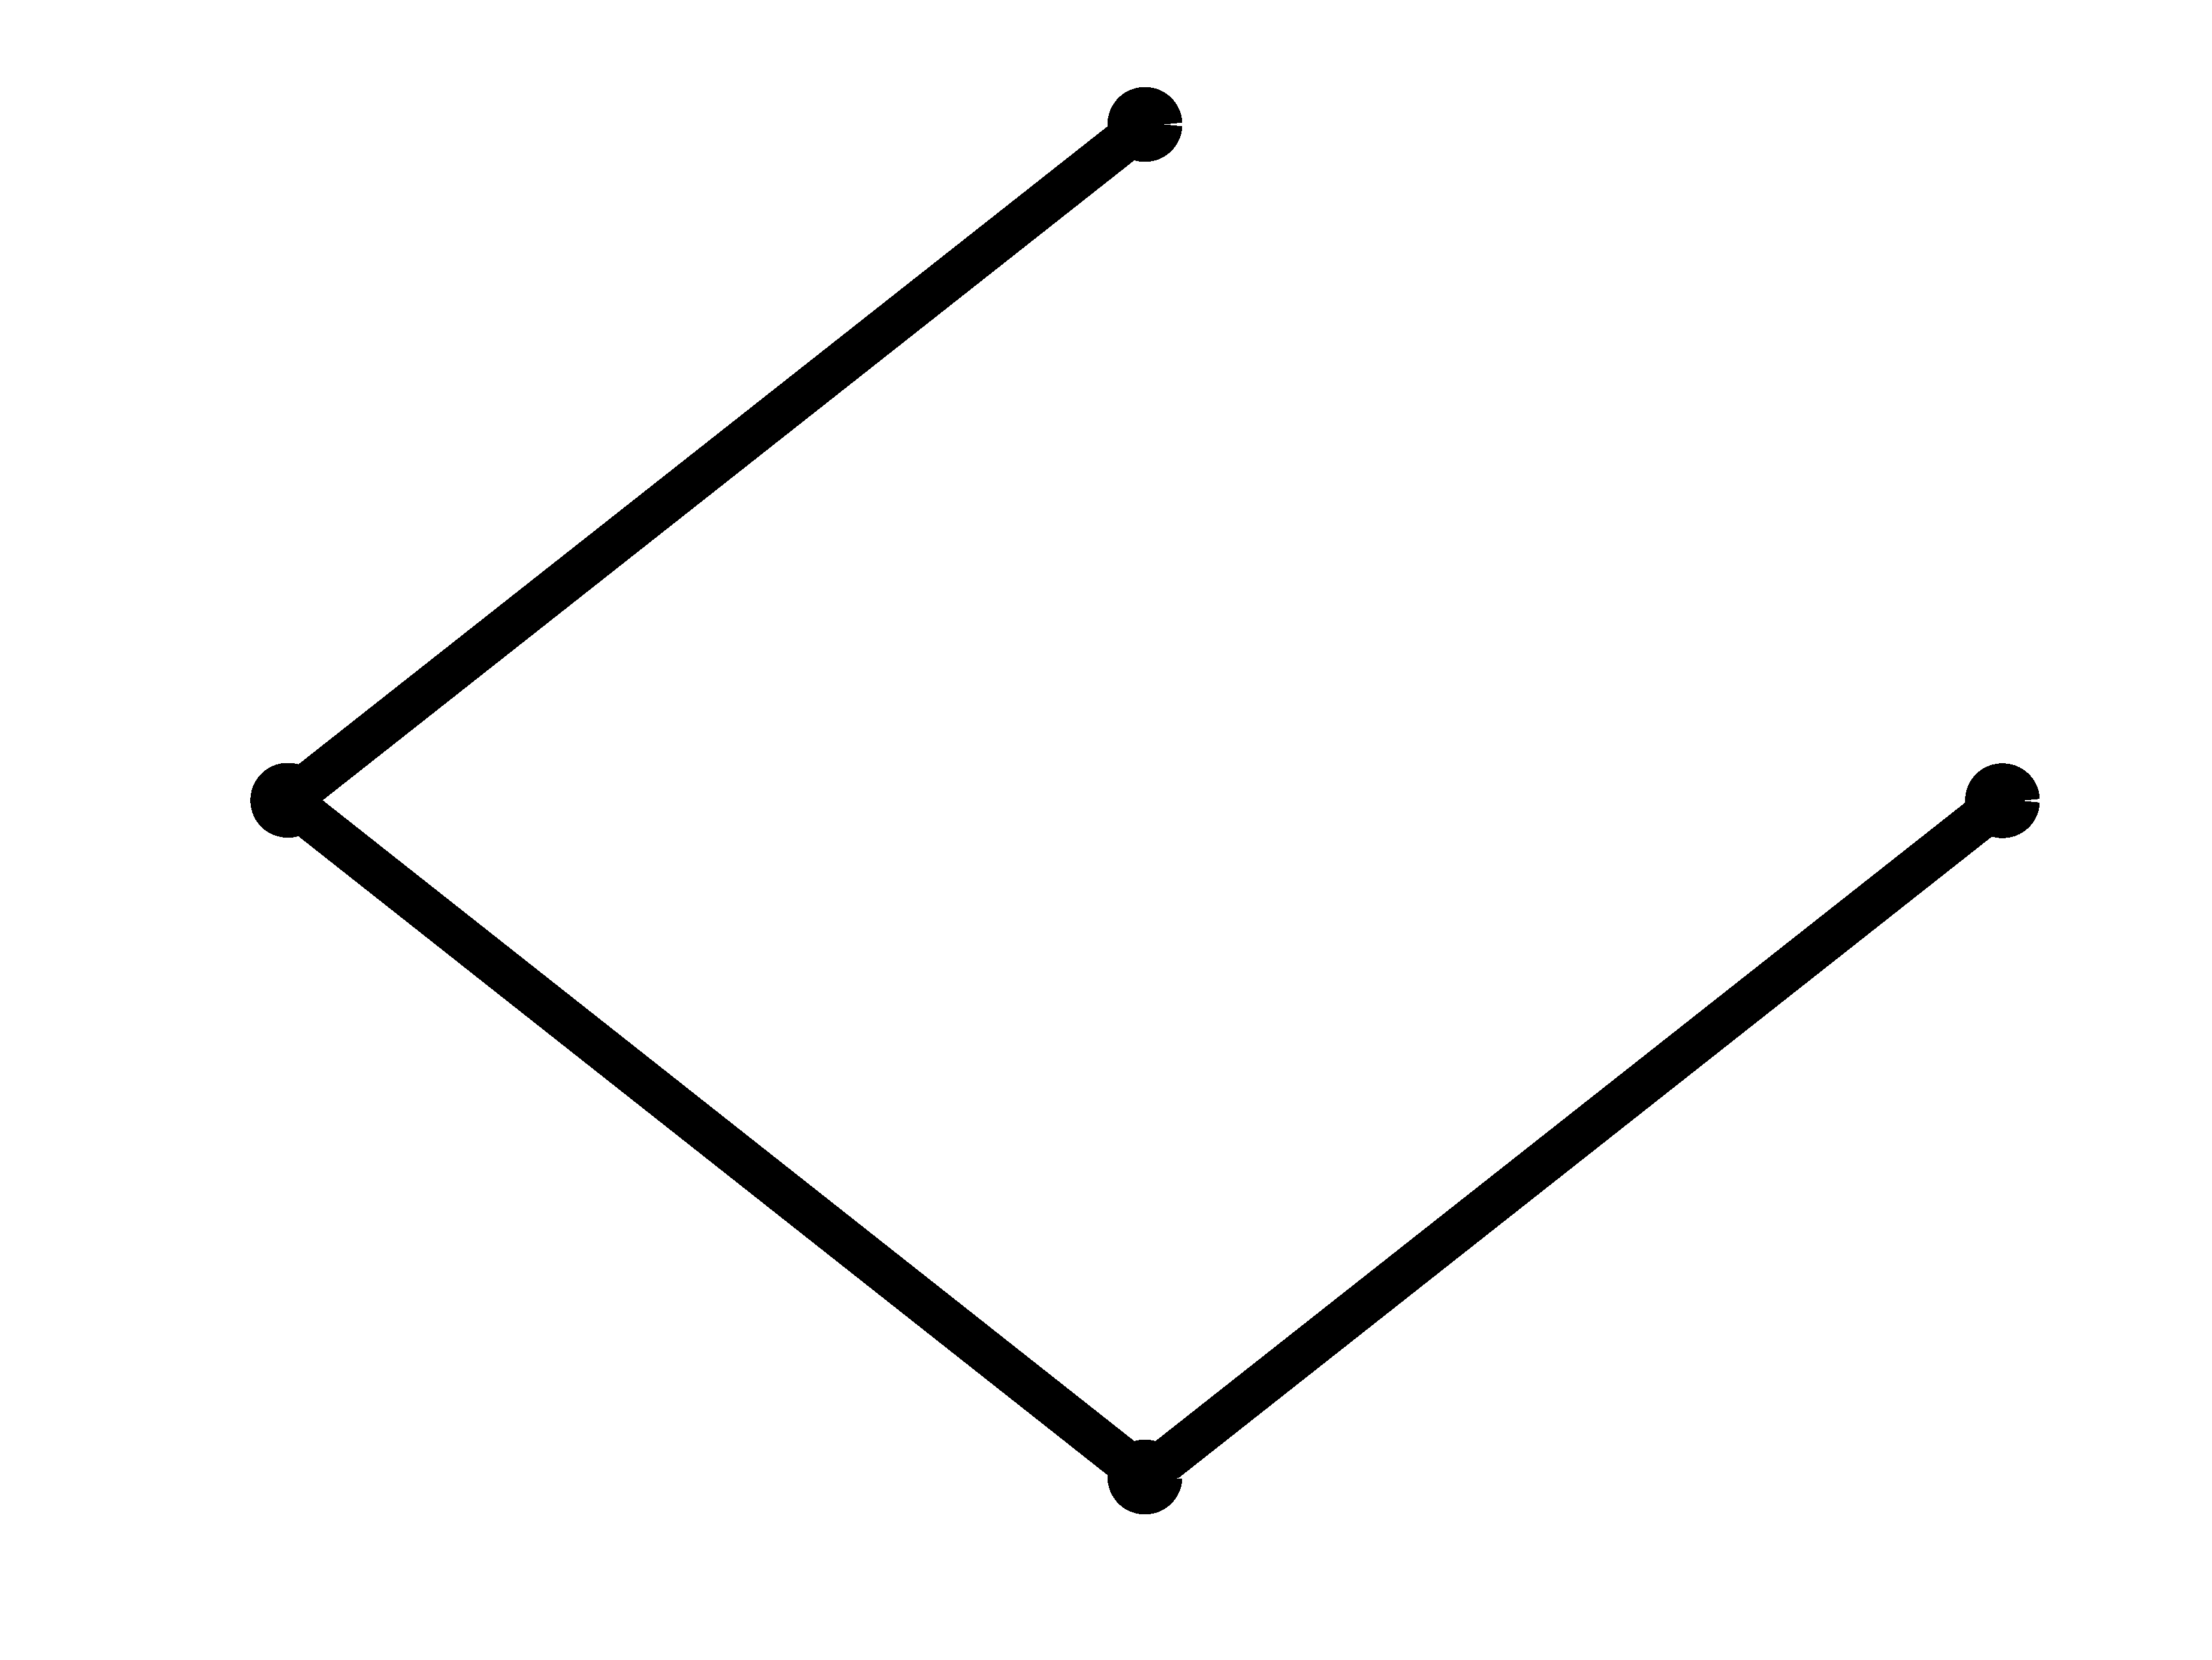
\epsfig{file =
      ../Figures/Motif-Chain4.eps, clip=, width=4cm, height=4cm}
  \end{tabular} & 
  \begin{tabular}{c} Loop: \end{tabular} & 
  \begin{tabular}{c} \hspace{-1.5cm} 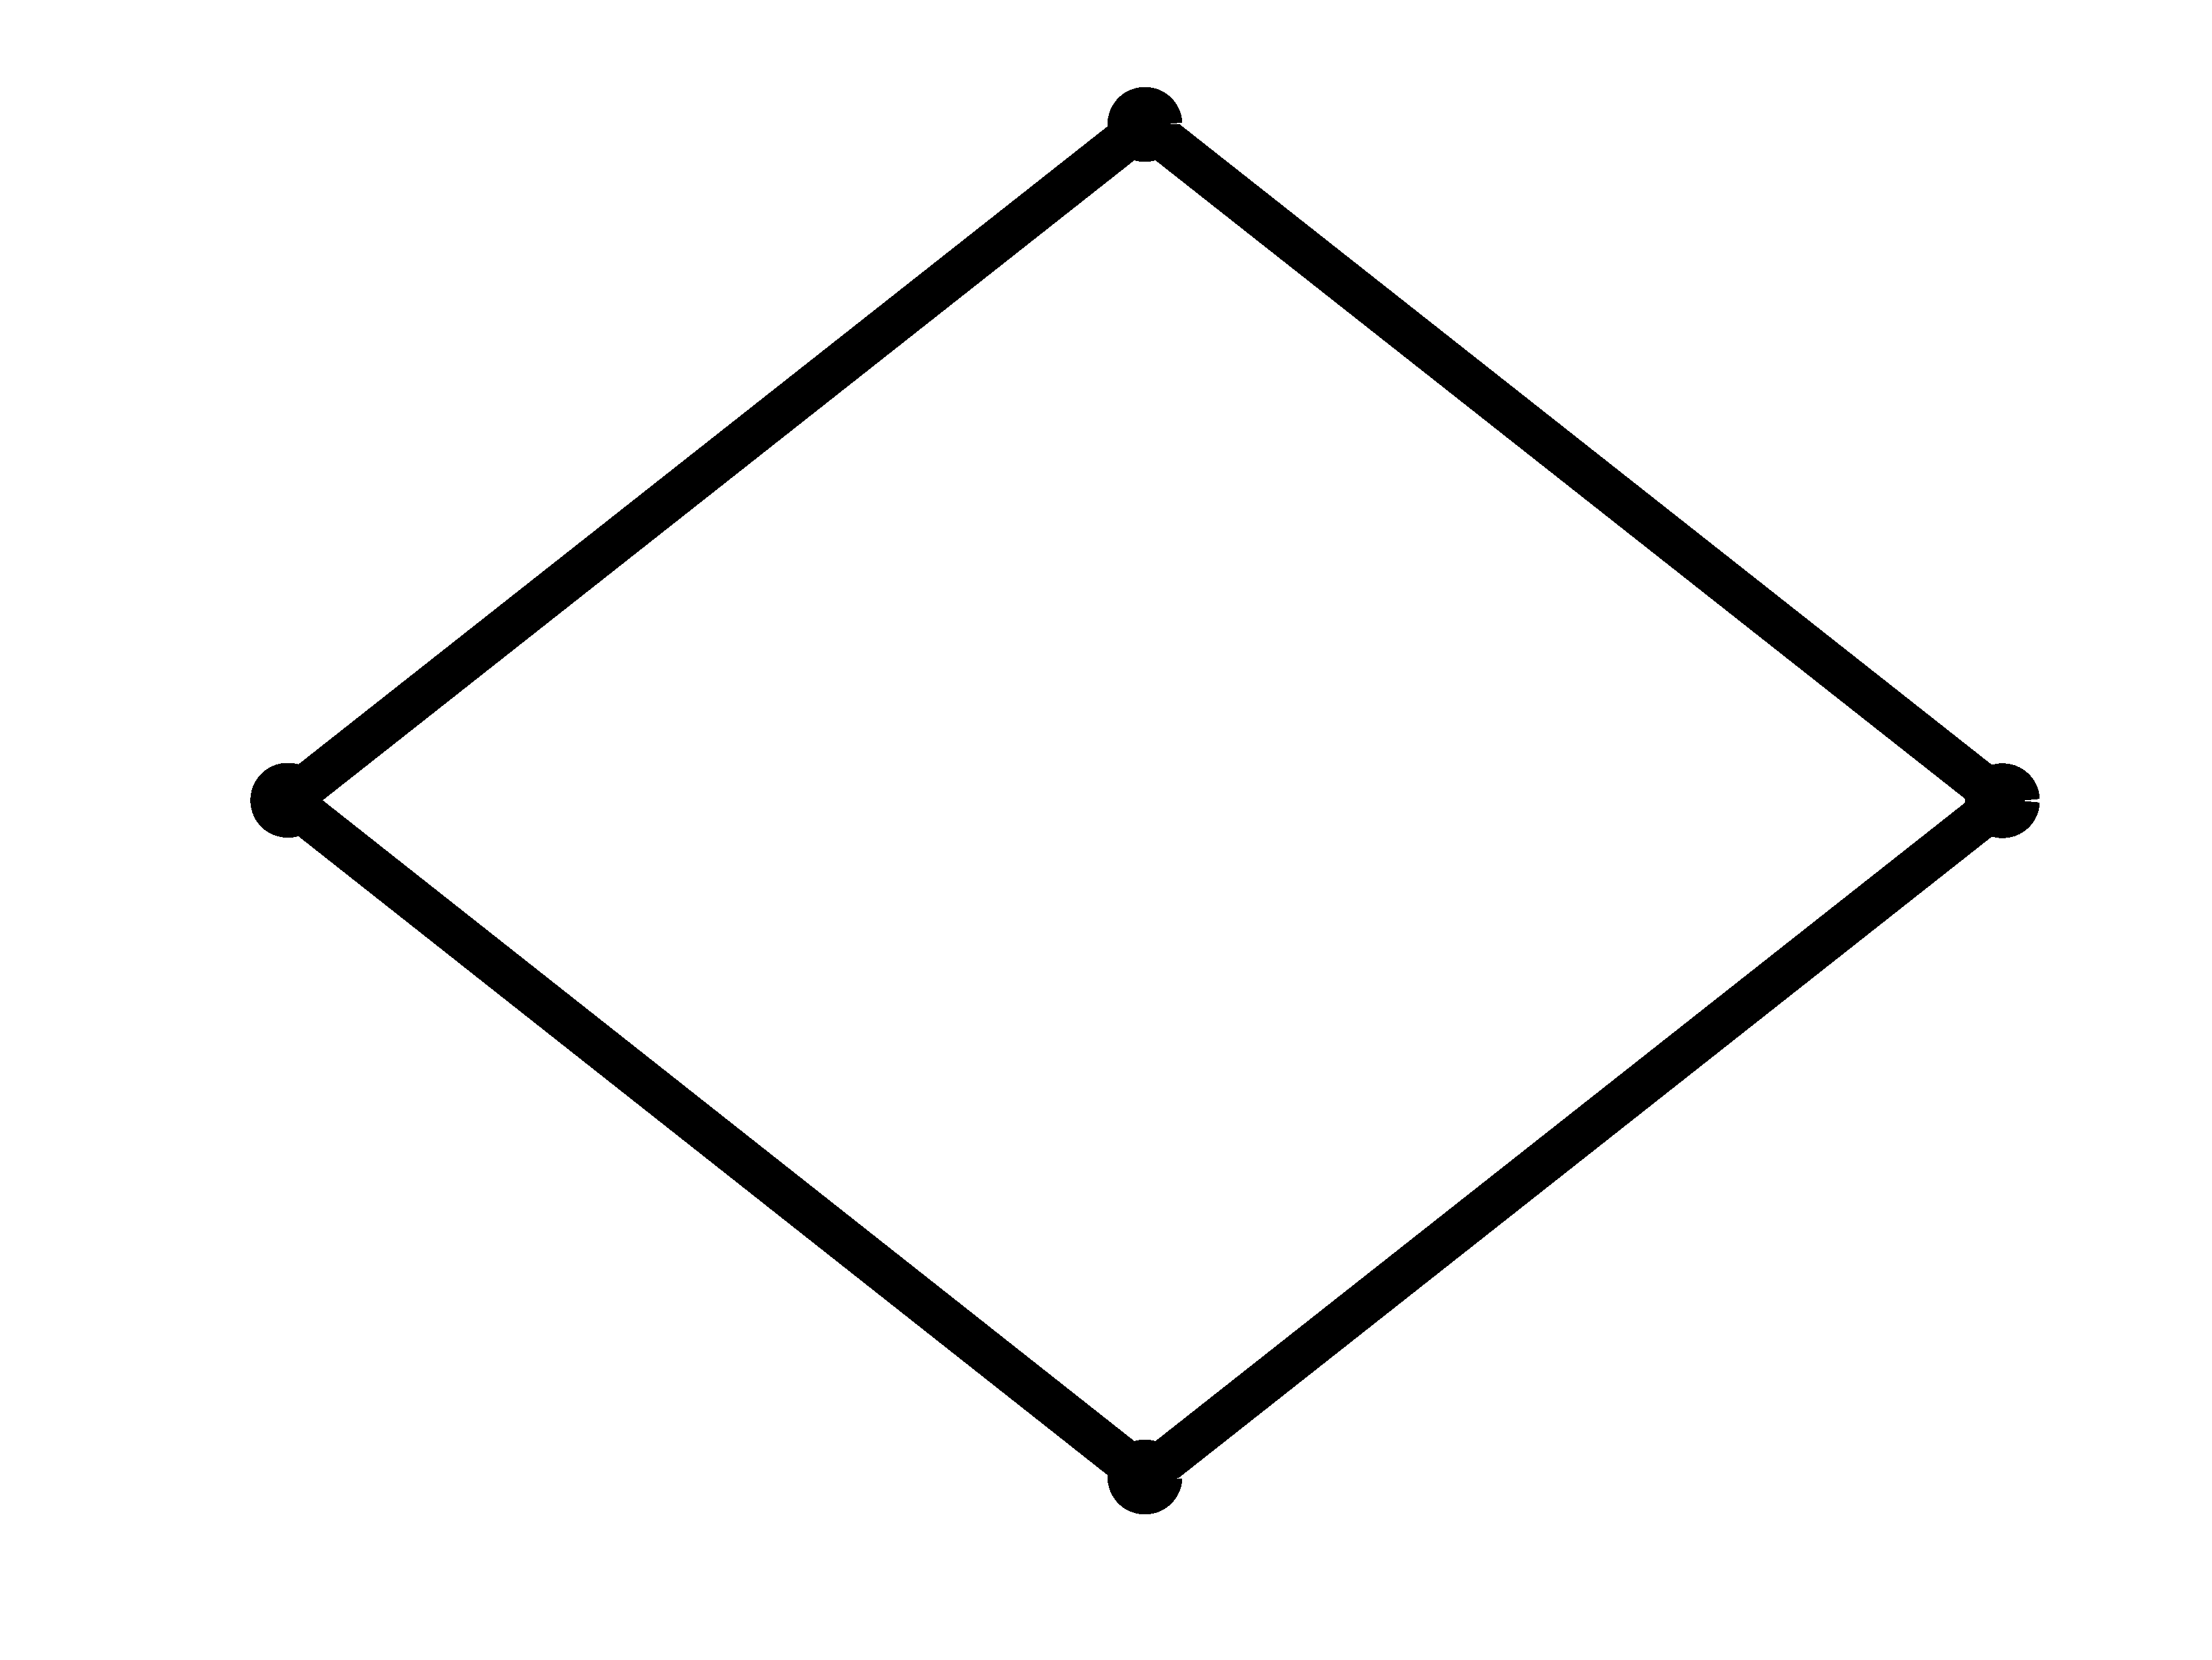
\epsfig{file =
      ../Figures/Motif-Square.eps, clip=, width=4cm, height=4cm}
  \end{tabular} & 
  \begin{tabular}{c} Hub: \end{tabular} & 
  \begin{tabular}{c} \hspace{-1.5cm} 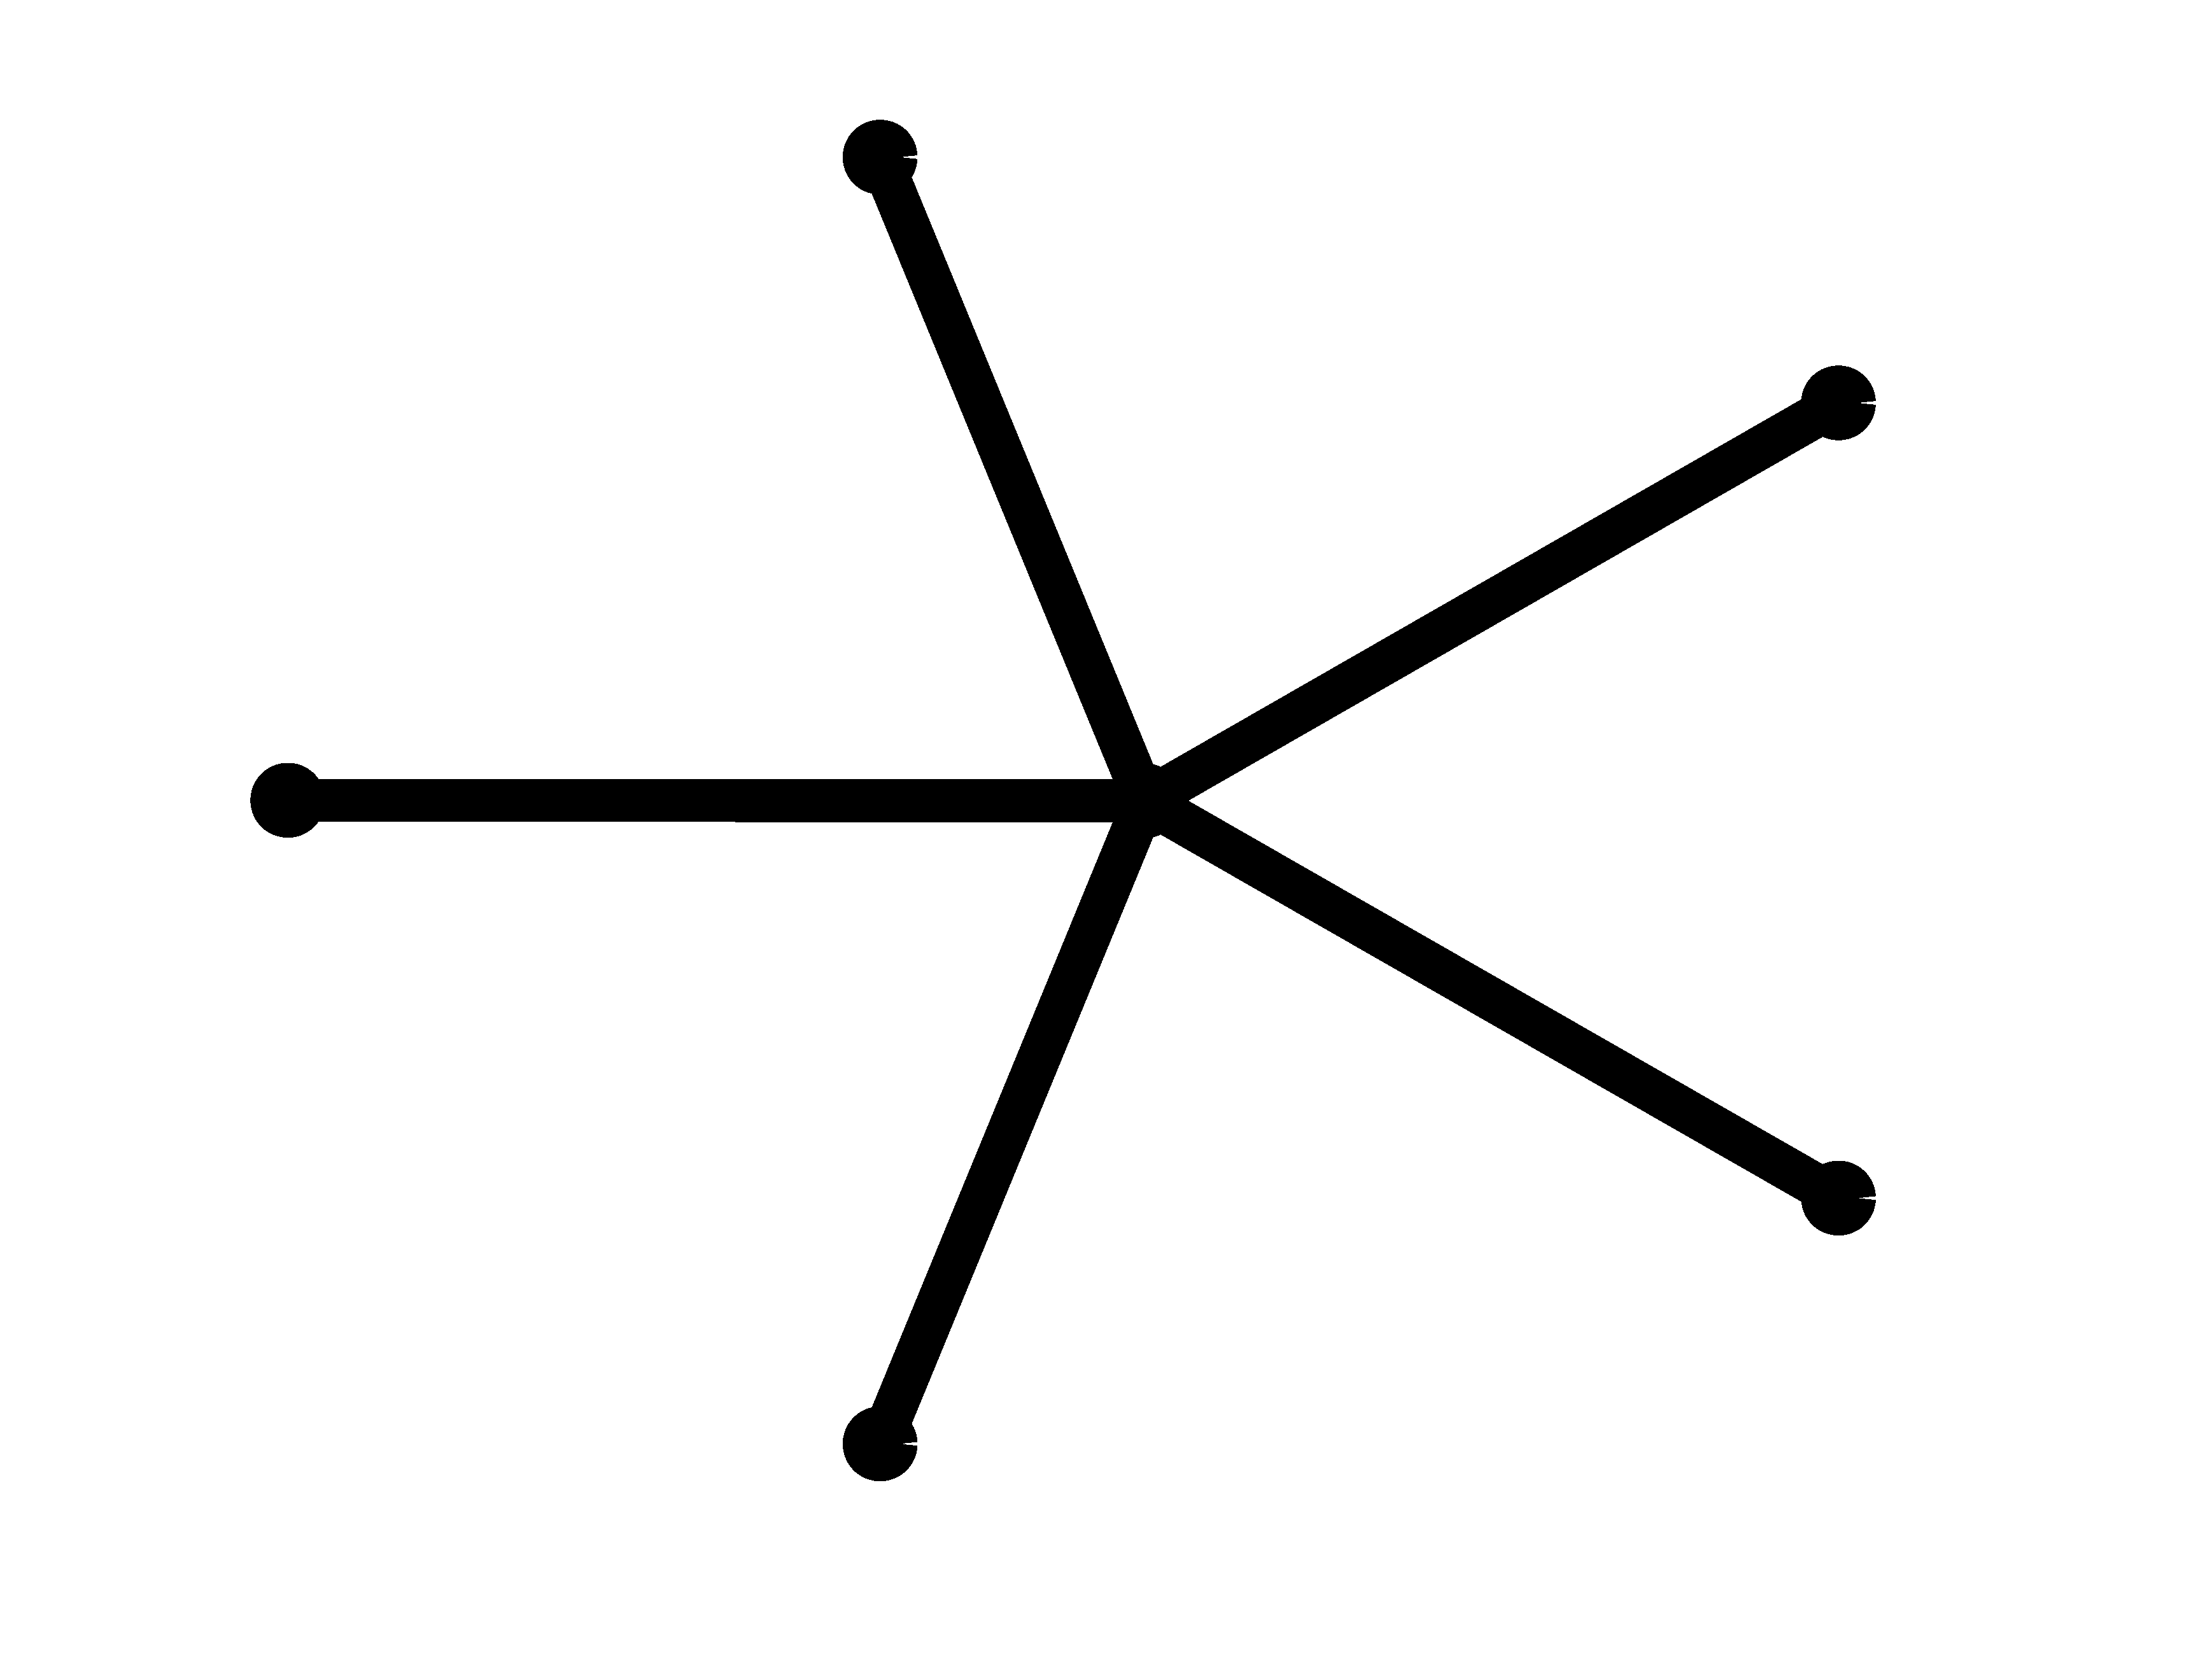
\epsfig{file =
      ../Figures/Motif-Star5.eps, clip=, width=4cm, height=4cm}
  \end{tabular}   
\end{tabular}
$$
For a given motif $\mbf$, we denote its count
$$
N_{\mbf}(G) = \mbox{number of occurrences of the motif $\mbf$ in the
  graph $G$}
$$
\paragraph{Question:} In a graph $G$ of size $n=200$, the motif $\mbf$
is observed $N_{\mbf}^{\mbox{obs}} = 20$ times. Is it \paragraph{exceptional}?

%%%%%%%%%%%%%%%%%%%%%%%%%%%%%%%%%%%%%%%%%%%%%%%%%%%%%%%%%%%%%%%%%%%%%%%%
\newpage
\section{Moments of the count}

\hspace{-2cm}
\begin{tabular}{cc}
  \begin{tabular}{p{12cm}}
    In the ERMG framework, for random graph $G$ with size $n$,
    proportions $\alpha_q$'s and connexion probabilities
    $\pi_{q\ell}$'s, we can calculate:
    \begin{itemize}
    \item the \paragraph{expected count $\Esp N_{\mbf}(G)$}, 
    \item the \paragraph{variance of the count $\Var N_{\mbf}(G)$}.
    \end{itemize}
    \\
    This calculation is based on the expected count of all the possible
    overlaps of the motif $\mbf$.
    \\ \\ \\
%     \paragraph{On the right:} All possible overlaps with 2 nodes for the
%     loop with 4 nodes ($\square$). 
    \paragraph{On the right:} All possible overlaps with 3 nodes for the
    star with 4 spikes: \\
    \begin{tabular}{cc}
      \begin{tabular}{c} $\mbf = $ \end{tabular} & 
      \begin{tabular}{c} \hspace{-2cm}     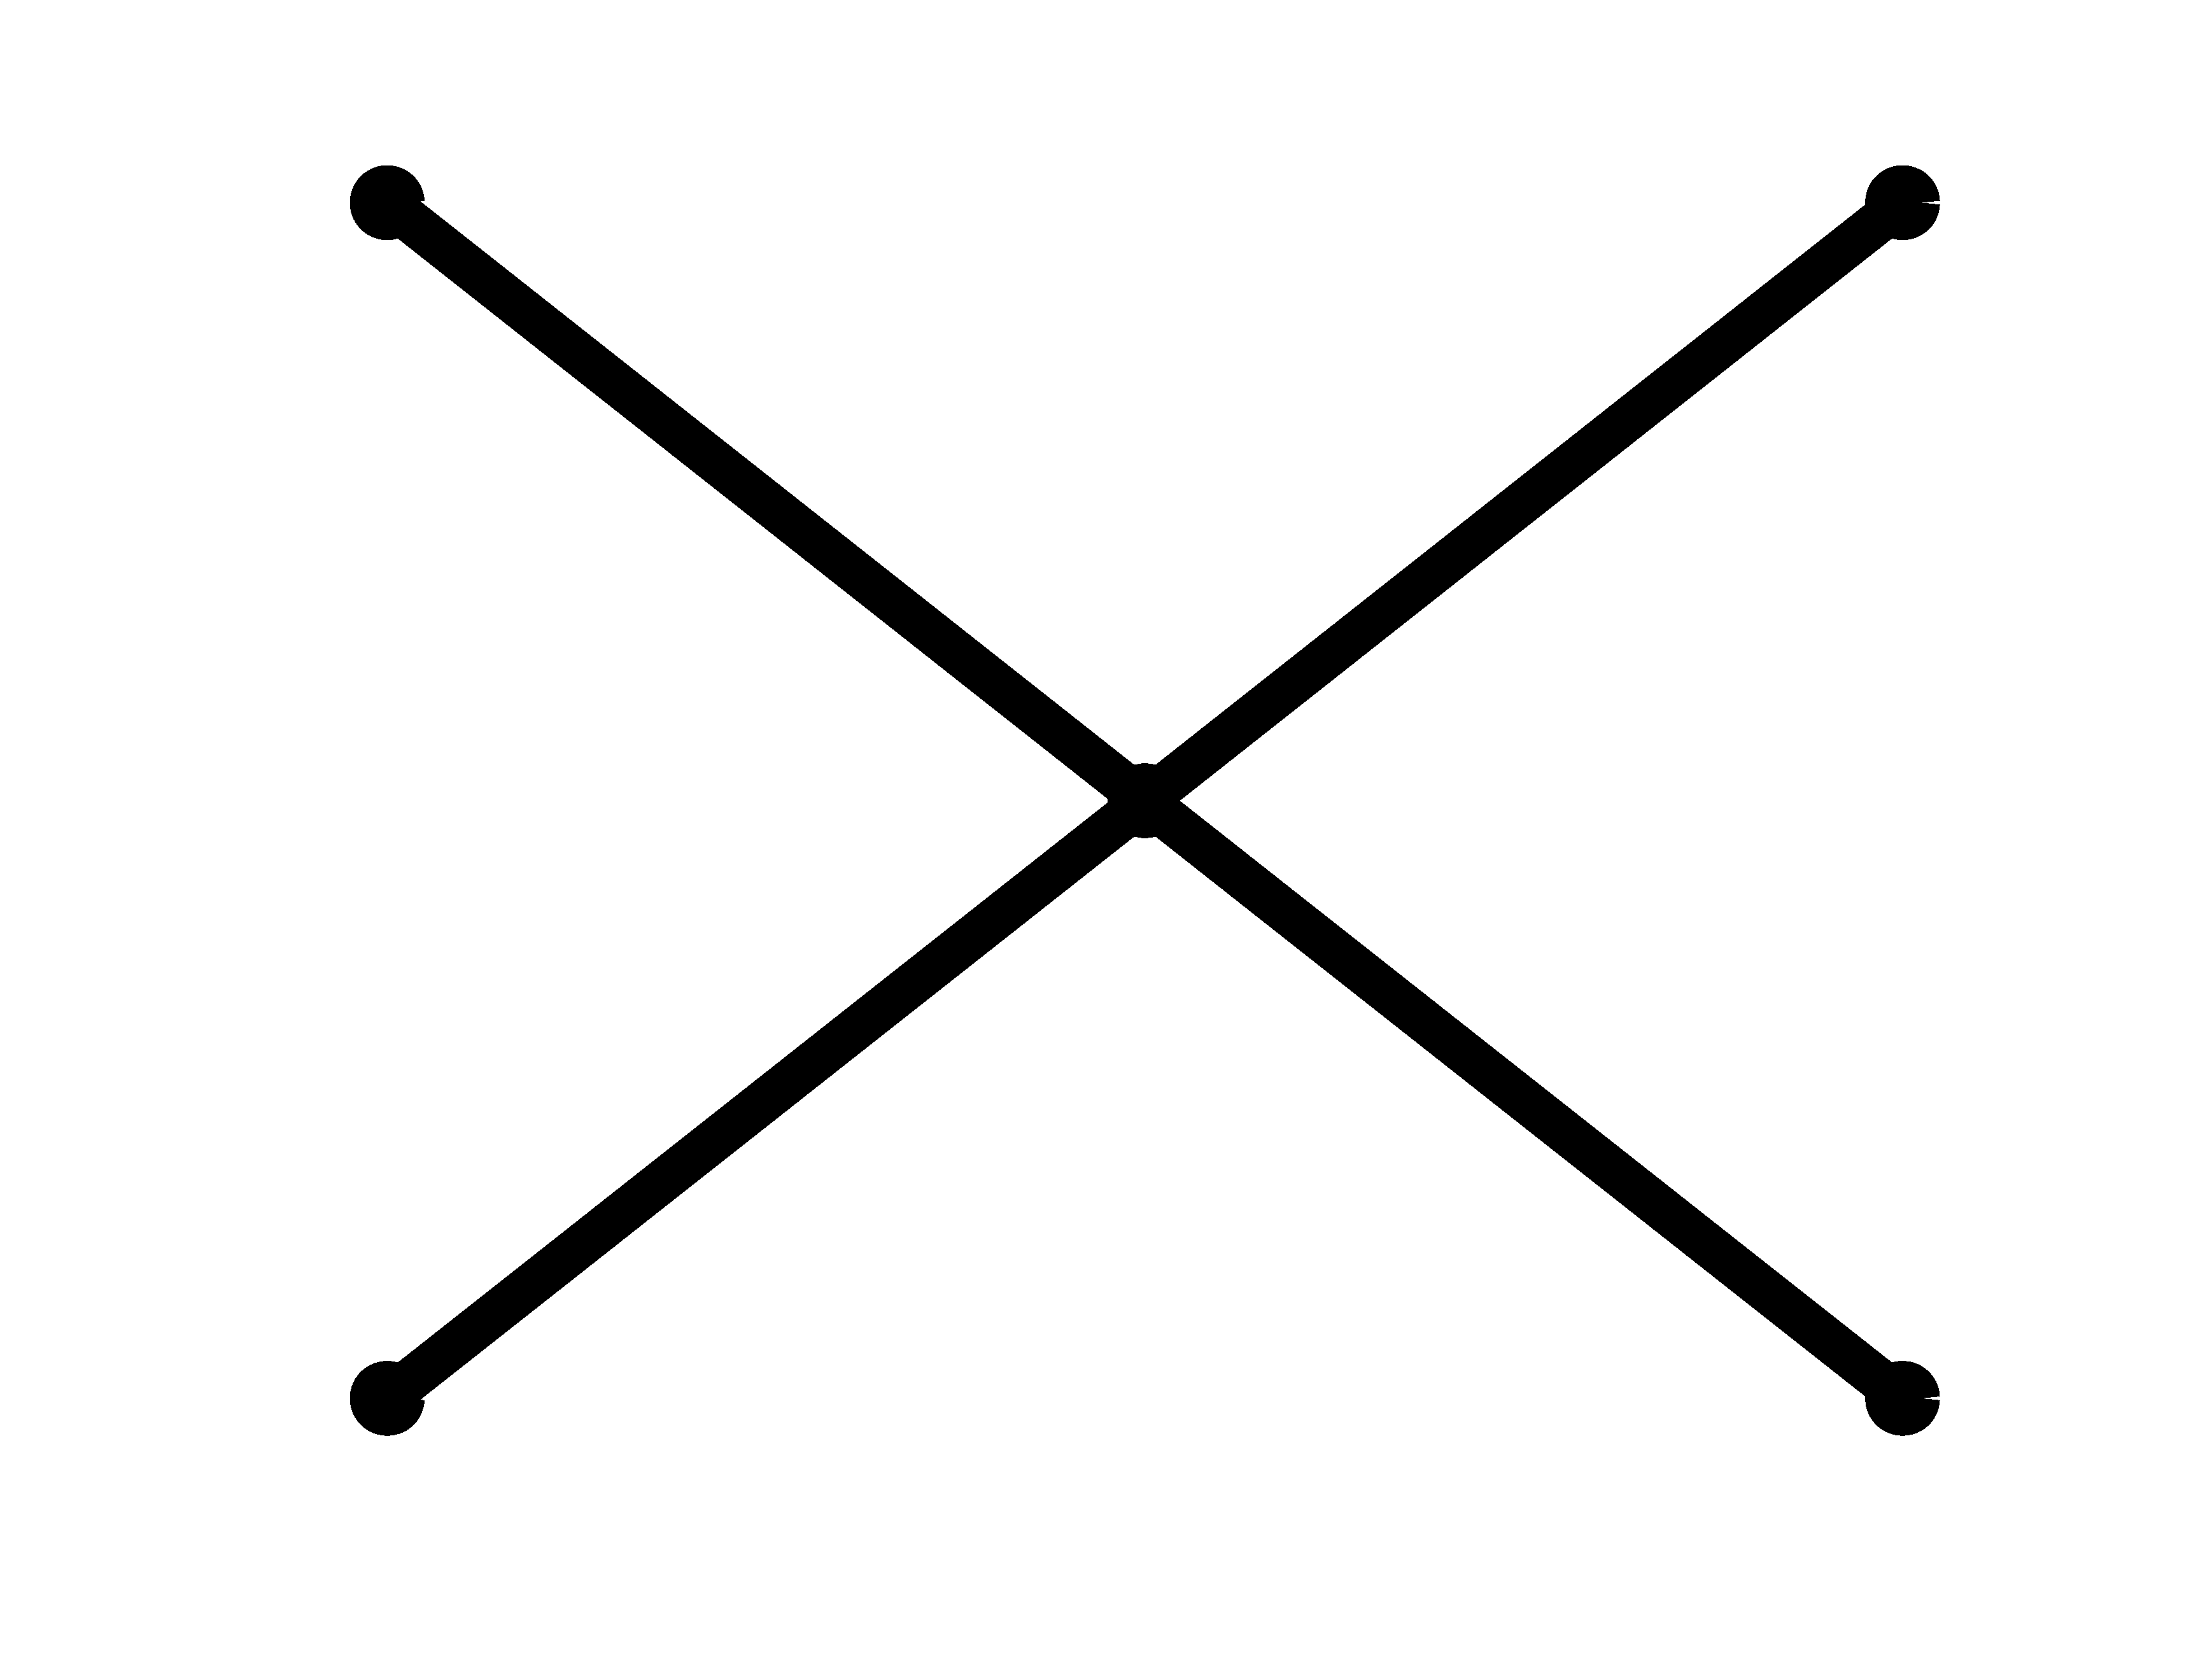
\epsfig{file =
          ../Figures/Motif-Star4.eps, clip=, width=2cm, height=2cm}
      \end{tabular}   
    \end{tabular}   
  \end{tabular}
  &
  \begin{tabular}{c}
%     \epsfig{file=
%       /RECHERCHE/RESEAUX/Motifs/FIGURES/MotifSquare-Recouv2.eps,
%       clip=, angle=270, width=12cm, height=6cm}
    \epsfig{file=
      /RECHERCHE/RESEAUX/Motifs/FIGURES/MotifStar4-Recouv3.eps,
      clip, width=10cm, height=15cm}
  \end{tabular}
\end{tabular}

%%%%%%%%%%%%%%%%%%%%%%%%%%%%%%%%%%%%%%%%%%%%%%%%%%%%%%%%%%%%%%%%%%%%%%%%
\newpage
\section{Approximate distribution of the count}

Based on simulations and analogy with motif statistics in sequences,
we propose to use the \paragraph{compound Poisson distribution}
(Polya-Aepply) to approximate the distribution of $N_{\bf m}$.

The parameters of this distribution are derived from $\Esp N_{\bf m}$
and $\Var N_{\bf m}$.

\hspace{-2cm}
\begin{tabular}{cc}
  \begin{tabular}{p{12cm}}
    \paragraph{Example:}  
    Distribution of the number of loops with 4 nodes ($\square$) 
    in a graph of size $n=200$, 
    under ERMG model with $Q=2$ groups and parameters 
    $$
    \alphabf = [\begin{array}{cc} 0.9 &  0.1 \end{array} ],
    \Pibf = \left[ \begin{array}{cc}
        0.004 & 0.037 \\ 
        0.037 & 0.004
      \end{array} \right].
    $$ 
  \end{tabular}
  &
  \hspace{-1.3cm}
  \begin{tabular}{c}
    \epsfig{file=/RECHERCHE/RESEAUX/Motifs/FIGJJD-150506/fig11_200.eps, 
      bbllx=332, bblly=211, bburx=515, bbury=304, width=12cm,
      height=7cm, clip=} \\
    \textred{\bf --} Gaussian, \textgreen{\bf --} Compound Poisson, 
%    \epsfig{file=
%        /RECHERCHE/RESEAUX/Motifs/FIGURES/DistStar4.eps, clip=,
%        width=14cm, height=12cm} 
   \end{tabular}
\end{tabular}
% The motif $\mbf = \square$ may occur at $\coefbin{200}{4} = 65\;10^6$
% positions. \\
We get 
$$
\Esp N_{\bf m} = 7.3, \qquad \Var N_{\bf m} = 21.7
$$
Suppose we observe 20 occurrences: $ \Pr\{N_{\bf m} \geq 20) = 1.7
\%$. 


%%%%%%%%%%%%%%%%%%%%%%%%%%%%%%%%%%%%%%%%%%%%%%%%%%%%%%%%%%%%%%%%%%%%%%%%
\newpage
\chapter{Conclusions}

\paragraph{Past.} 
\begin{itemize}
\item \vspace{-0.5cm} The ERMG model is a flexible generalization of
  the ER model and a promising alternative to the scale-free model.
\item \vspace{-0.5cm} It seems to fit well several real-world networks
  %(Airport network, Enzyme network in bacteria, etc.).
\item \vspace{-0.5cm} It is properly defined, so its properties can be
  properly studied.
\end{itemize}

\paragraph{Future.}
\begin{itemize}
\item \vspace{-0.5cm} Study the probabilistic properties of the ERMG
  model (diameter, sampling properties, etc).
\item \vspace{-0.5cm} Study the statistical properties of the
  estimates; Derive a relevant criterion to select the number of
  groups.
\item \vspace{-0.5cm} Extension to valued graphs: $X_{ij}$ not only
  0/1, but some measure of the connection intensity.
\end{itemize}


%%%%%%%%%%%%%%%%%%%%%%%%%%%%%%%%%%%%%%%%%%%%%%%%%%%%%%%%%%%%%%%%%%%%%%%%
%%%%%%%%%%%%%%%%%%%%%%%%%%%%%%%%%%%%%%%%%%%%%%%%%%%%%%%%%%%%%%%%%%%%%%%%
%%%%%%%%%%%%%%%%%%%%%%%%%%%%%%%%%%%%%%%%%%%%%%%%%%%%%%%%%%%%%%%%%%%%%%%%
%%%%%%%%%%%%%%%%%%%%%%%%%%%%%%%%%%%%%%%%%%%%%%%%%%%%%%%%%%%%%%%%%%%%%%%%
\end{document}
%%%%%%%%%%%%%%%%%%%%%%%%%%%%%%%%%%%%%%%%%%%%%%%%%%%%%%%%%%%%%%%%%%%%%%%%
%%%%%%%%%%%%%%%%%%%%%%%%%%%%%%%%%%%%%%%%%%%%%%%%%%%%%%%%%%%%%%%%%%%%%%%%
%%%%%%%%%%%%%%%%%%%%%%%%%%%%%%%%%%%%%%%%%%%%%%%%%%%%%%%%%%%%%%%%%%%%%%%%
%%%%%%%%%%%%%%%%%%%%%%%%%%%%%%%%%%%%%%%%%%%%%%%%%%%%%%%%%%%%%%%%%%%%%%%%

